\documentclass[12pt]{article}

\usepackage{lineno}


\usepackage[hmargin=1.5cm,vmargin=1.5cm]{geometry}

\usepackage[affil-it]{authblk}
\usepackage[percent]{overpic}
\usepackage{float}
\usepackage{color}
\usepackage{hyperref}
\usepackage[numbers,sort&compress]{natbib}

\title{Beam test of the silicon timing for use in calorimetry.}

\author[1]{A.~Apresyan}
\author[2]{G.~Bolla}
\author[1]{A.~Bornheim}
\author[3]{H.~Kim}
\author[2]{S.~Los}
\author[1]{C.~Pena}
\author[2]{E.~Ramberg}
\author[2]{A.~Ronzhin}
\author[1]{M.~Spiropulu}
\author[1]{S.~Xie}
\affil[1]{California Institute of Technology, Pasadena, CA, USA}
\affil[2]{Fermi National Accelerator Laboratory, Batavia, IL, USA}
\affil[3]{University of Chicago, Chicago, IL,  USA}

\date{}

\begin{document}
\linenumbers
\maketitle

\abstract{ The high luminosity upgrade of the Large Hadron Collider (HL-LHC) at
CERN is expected to provide instantaneous luminosities of $5\times 10^{34}$
cm$^{-2}$ s$^{-1}$. The high luminosities expected at the HL-LHC will be
accompanied by a factor of $5$ to $10$ more pileup compared with LHC conditions
in $2015$, causing general confusion for particle identification and event
reconstruction. Precision timing allows to extend calorimetric measurements into
such a high density environment by subtracting the energy deposits from pileup
interactions. Calorimeters employing silicon as the active component have
recently become a popular choice for the HL-LHC and future collider experiments
which face very high radiation environments. In this article, we present studies
of basic calorimetric and precision timing measurements using a prototype composed of
tungsten absorber and silicon sensor as the active medium. We show that for
the bulk of electromagnetic showers induced by electrons in the range of
$20$~GeV to $30$~GeV, we can achieve time resolutions better than $25$~ps per
single pad sensor. 

\section{Introduction} 

Future colliders, including the high luminosity upgrade of the Large
Hadron Collider (HL-LHC) at CERN, will require improvements to the instantaneous
luminosity by an order of magnitude or more compared to what has been achieved
at the LHC so far. With the increased instantaneous luminosity the rate of
simultaneous interactions per bunch crossing (pileup) is projected to reach an
average of 140 to 200. The large amount of pileup increases the likelihood of
confusion in the reconstruction of events of interest, due to the contamination
from particles produced in different pileup interactions. The ability to
discriminate between jets produced in the events of interests, especially those
associated with the vector boson fusion processes, and jets produced by pileup
interactions will be degraded. The missing transverse energy resolution will
deteriorate, and several other physics object performance metrics will suffer.

One way to mitigate the pileup confusion effects, complementary to precision
tracking methods, is to perform a time of arrival measurement associated with a
particular layer of the calorimeter, allowing for a time assignment for 
charged particles and photons. Such a measurement with a precision of about
20-30 ps, when unambiguously associated to the corresponding energy measurement,
will reduce the effective amount of pileup by a factor of 10, given that the
spread in collision time of the pileup interactions at HL-LHC is foreseen to be
approximately 200~ps. The association of the time measurement with the energy
measurement is crucial, and leads to a prototype design that calls for the time
and energy measurements to be performed in the same detector element. Since both
the energy and time measurement are performed in the same detector element, once
an energy deposit is identified as originating from a pileup interaction, it can
be unambiguously removed from event reconstruction.

Several alternative options to combine high resolution energy and timing
measurements for calorimetry have been reported in Refs.~\cite{Anderson:2015gha,
MCPFastCaloNIMA, Ronzhin2015288, Ronzhin201552, Brianza2015216}. In this
article, we describe the continuation of this program of study using a
calorimeter prototype employing a silicon pad sensor of $6\times 6$~mm$^2$ size
as the active element. Silicon-based calorimeters have recently become a popular
choice for future colliders due to the radiation hardness of silicon, and the
ability to construct highly granular detectors. An important example is the
forward calorimeter proposed for the CMS Phase 2 Upgrade~\cite{Butler:2020886}.
We study the timing properties of silicon-based calorimetery using a prototype
composed of tungsten absorber and a silicon sensor produced by
Hamamatsu~\cite{hamamatsu}. 

The paper is organized as follows. General silicon timing properties and bench
test results are described in Section~\ref{sec:siliconpad}. The test beam setup
and experimental apparatus are presented in Section~\ref{sec:tbeam}. The results
of the test beam measurements are presented in Section~\ref{sec:results}.
Sections~\ref{sec:discussion}~and~\ref{sec:conclusion} are devoted to discussion
and conclusion, respectively.


\section{General Properties of Silicon Timing and Bench Test Studies}
\label{sec:siliconpad}

For our measurements, we used a silicon sensor produced by
Hamamatsu~\cite{hamamatsu}. The thickness of the silicon was measured to be ~325
$\mu$m. The transverse size of the sensor is 6x6 mm$^2$. The negative bias
voltage was applied to the p-side of the silicon. The capacitance
of the silicon diode is measured as a function of the bias voltage
and shown in Figure~\ref{fig:SiliconDiode}. We observe that the silicon
is fully depleted above about $120$~V. Timing measurements are expected
to improve with larger bias voltage as the the carrier velocity increases.

The electric diagram of the silicon
diode connections is presented in Figure~\ref{fig:SiliconPad}. Attention was
paid to provide good filtering for bias voltage, to reduce ground loop effects, and
to minimize inductive loop for the signal readout. The timing characteristics
of the signal pulses are dominated primarily by properties of the
silicon sensor rather than the details of the circuit.

\begin{figure}[htbp] 
\centering
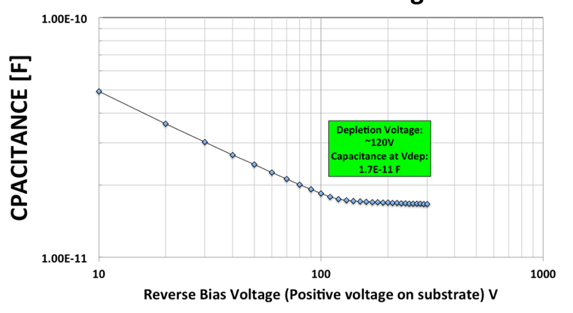
\includegraphics[width=0.45\textwidth]{plots/SiliconDiodeCV.png} 
\caption{The measured capacitance as a function of the applied bias voltage.} 
\label{fig:SiliconDiode} 
\end{figure} 

The silicon diode was placed inside a light-tight box of thickness $1.5$~cm,
which also provides electromagnetic shielding. The box is made of 0.2~mm steel.
The bias voltage was supplied to the circuitry by a cable with a balun filter,
terminated with an SHV connector. The silicon diode output signal is read out
through an SMA connector electrically connected to the box. The dark current was
measured at several values of the bias voltage. The maximum value of the dark
current was less than $1.0$~nA at $-500$~V, which is the largest bias voltage
used in the measurements reported in this paper. The silicon box and bench test
setup are presented in Figure~\ref{fig:SiliconPad}. 

\begin{figure}[htbp] 
\centering
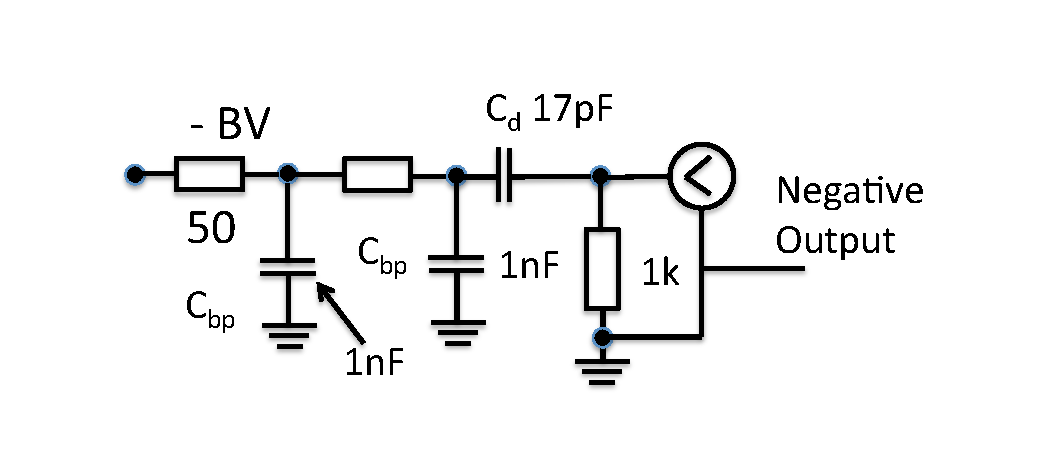
\includegraphics[width=0.60\textwidth]{plots/SiliconDiodeDiagram.pdf} 
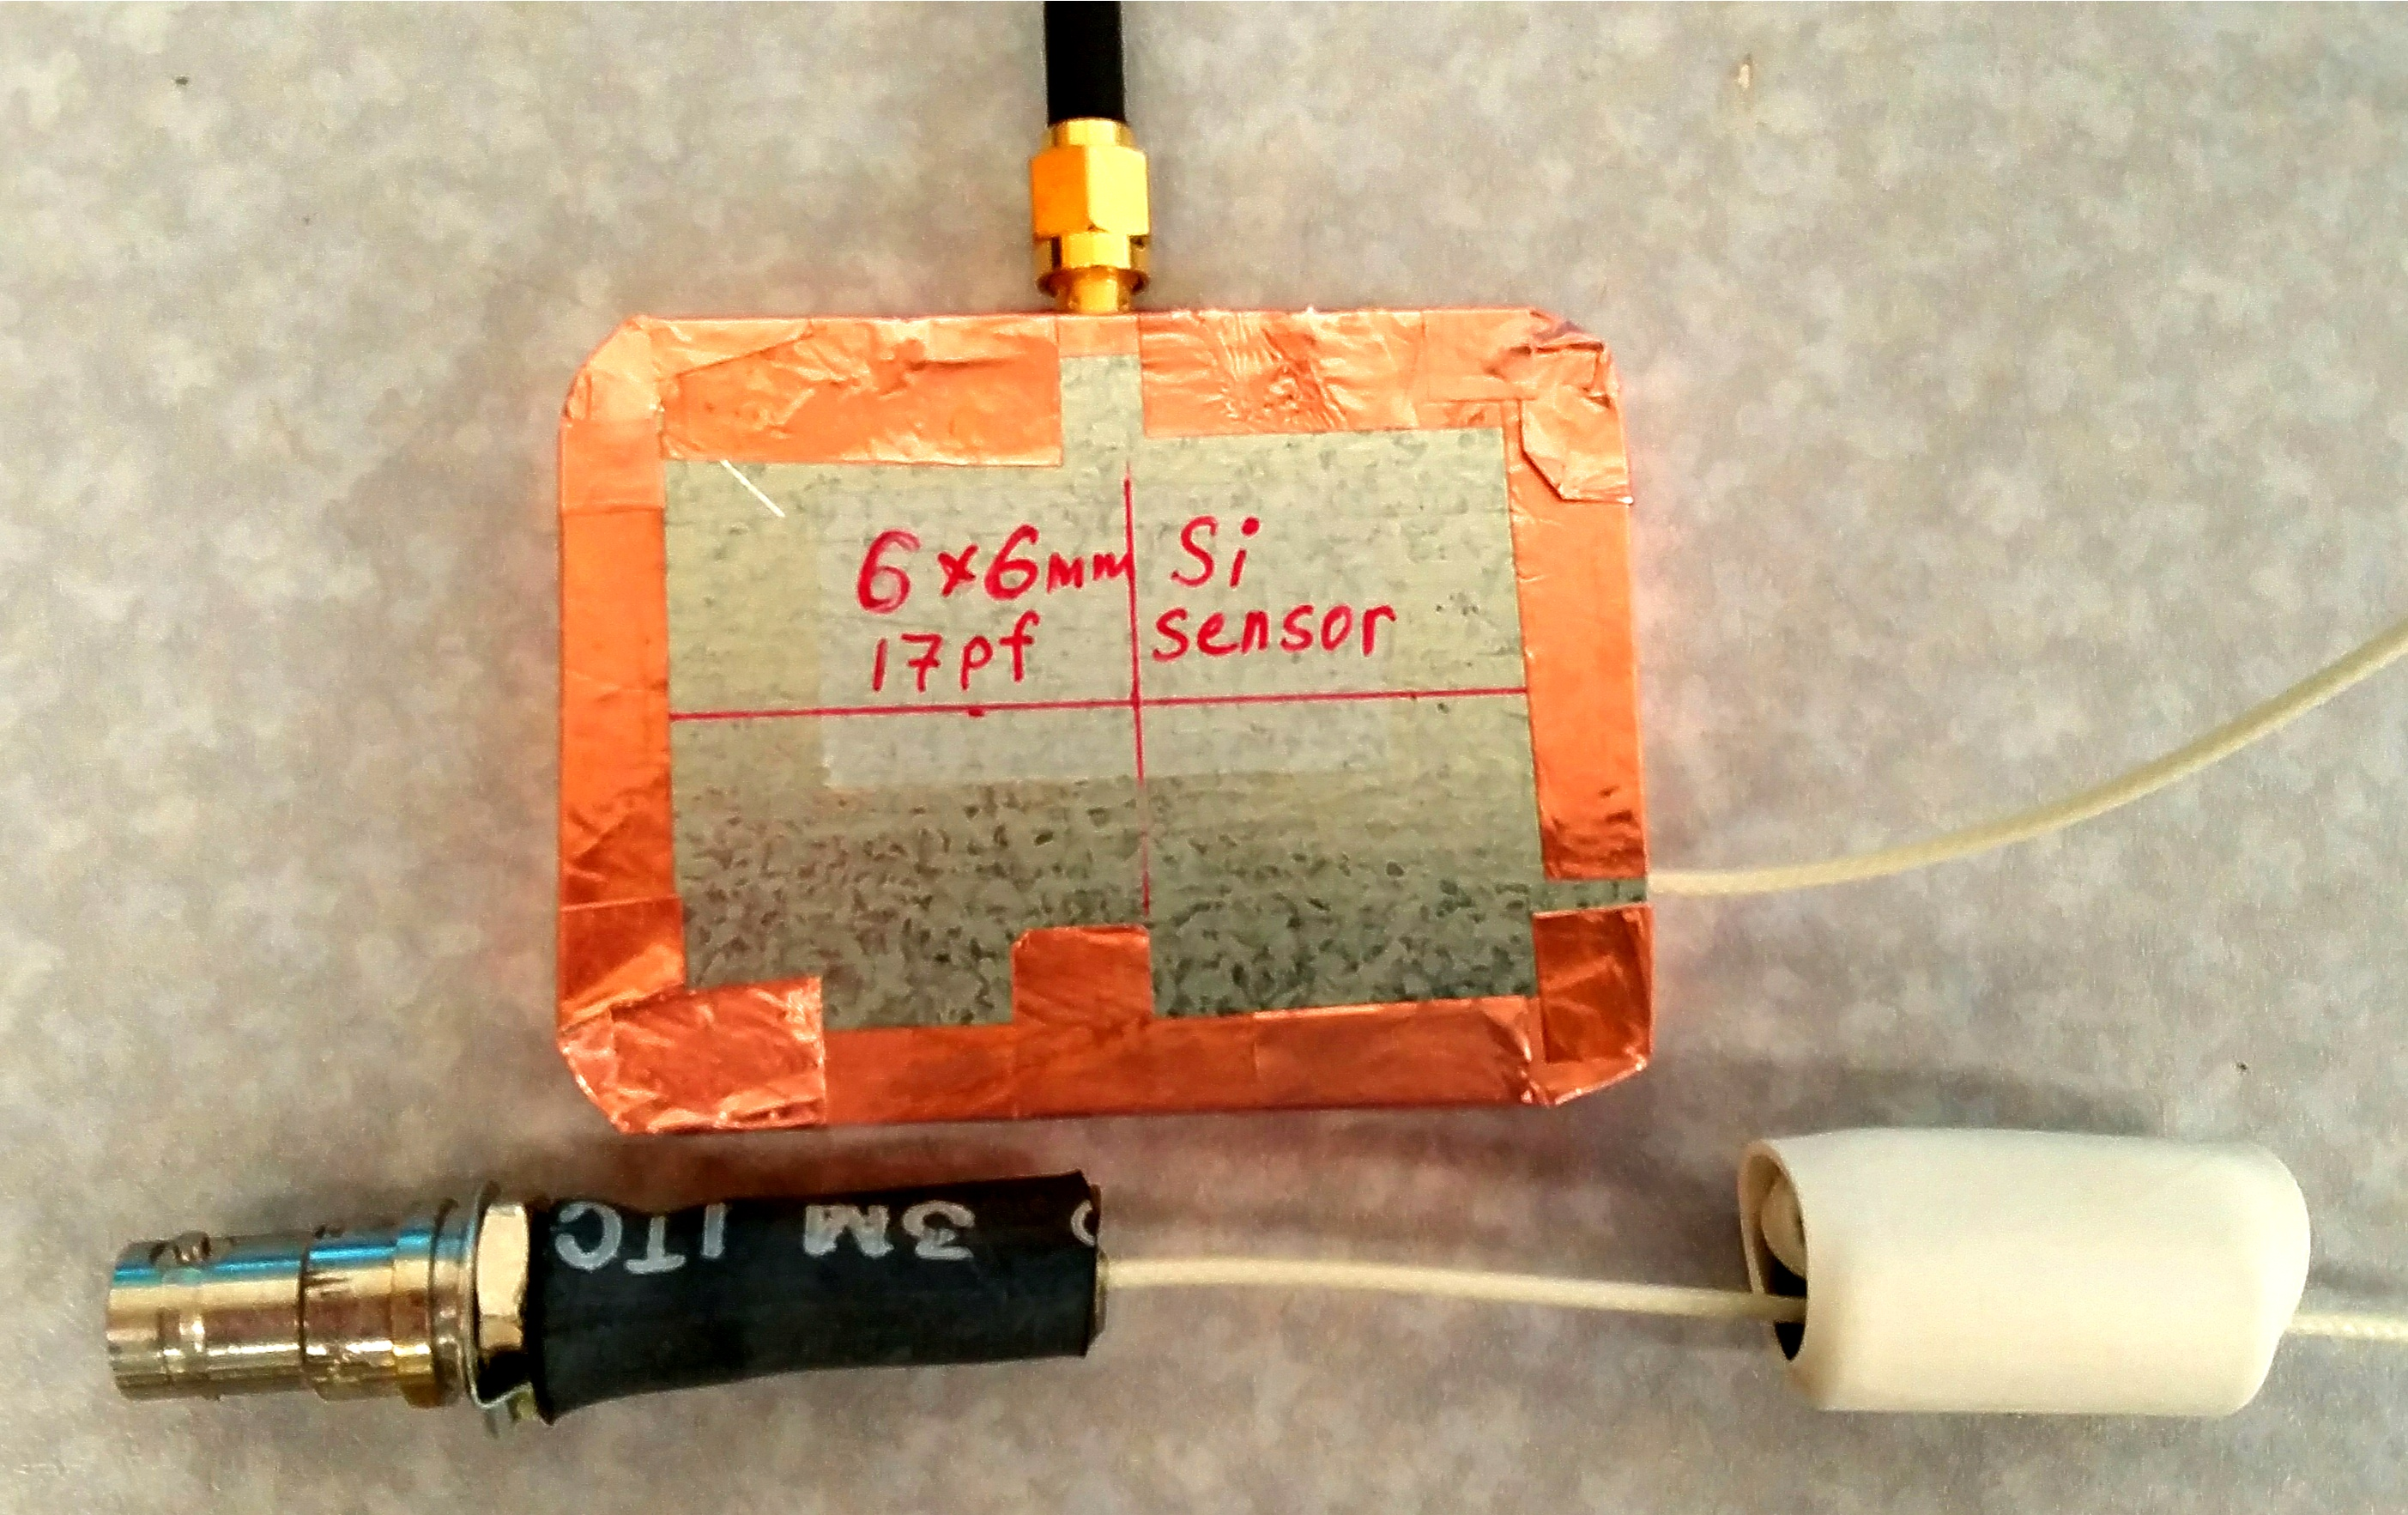
\includegraphics[width=0.39\textwidth]{plots/SiliconDiodeBox.jpg} 
\caption{The electric diagram for the silicon diode connections (left). External
view of the box with silicon diode, and the bias voltage connection is shown
below it (right).} 
\label{fig:SiliconPad} 
\end{figure} 

The signals from the silicon sensor were amplified by two fast and
high-bandwidth pre-amplifiers connected in series. The first amplifier is an
ORTEC VT120C pre-amplifier, and the second amplifier is a Hamamatsu C5595
amplifier. Using a pulse-generator, we measured the combined amplification gain
of the two amplifiers in series as a function of the input signal amplitude and
found some degree of non-linearity for typical signals produced by the silicon
sensor under study. The measured gain ranged from $200$ for signals with
amplitude around $0.15$~mV to $650$ for signals with amplitude around $10$~mV.

\section{Test-beam Setup and Experimental Apparatus }
\label{sec:tbeam}

We performed the test-beam measurements at the Fermilab Test-beam Facility
(FTBF) which provided a proton beam from the Fermilab Main Injector accelerator
at $120$~GeV, and secondary beams composed of electrons, pions, and muons of
energies ranging from $4$~GeV to $32$~GeV. A simple schematic diagram of the
experimental setup is shown in Figure~\ref{fig:BeamSchematicDiagram}. A small
plastic scintillator of transverse dimensions $1.8$~mm$\times 2$~mm is used as a
trigger counter to initiate the read out of the data acquisition (DAQ) system.
It is also used to constrain the transverse beam-spot to a small geometric area.
Next, we place a stack of tungsten absorbers of various thicknesses for
measurements of the longitudinal profile of the electromagnetic shower. The
silicon pad sensor is located within a metal box covered by copper foil, and is
placed immediately downstream of the absorber plates. Finally, a Photek 240
micro-channel plate photomultiplier detector~\cite{Anderson:2015gha,
MCPFastCaloNIMA, Ronzhin2015288,Ronzhin201552} is placed furthest downstream,
and serves to provide a very precise reference timestamp. Its precision was
previously measured to be less than $10$~ps~\cite{MCPShowerMaxPaper}. 
A photograph showing the various
detector components is presented in Figure~\ref{fig:BeamPhotoDiagram}. A
differential Cherenkov counter is located further upstream of our experimental
setup and provides additional particle identification capability. More
details of the experimental setup are described in our previous studies using
the same experimental facility in references~\cite{Anderson:2015gha,
MCPFastCaloNIMA, Ronzhin2015288,Ronzhin201552}.

\begin{figure}[htbp] 
\centering
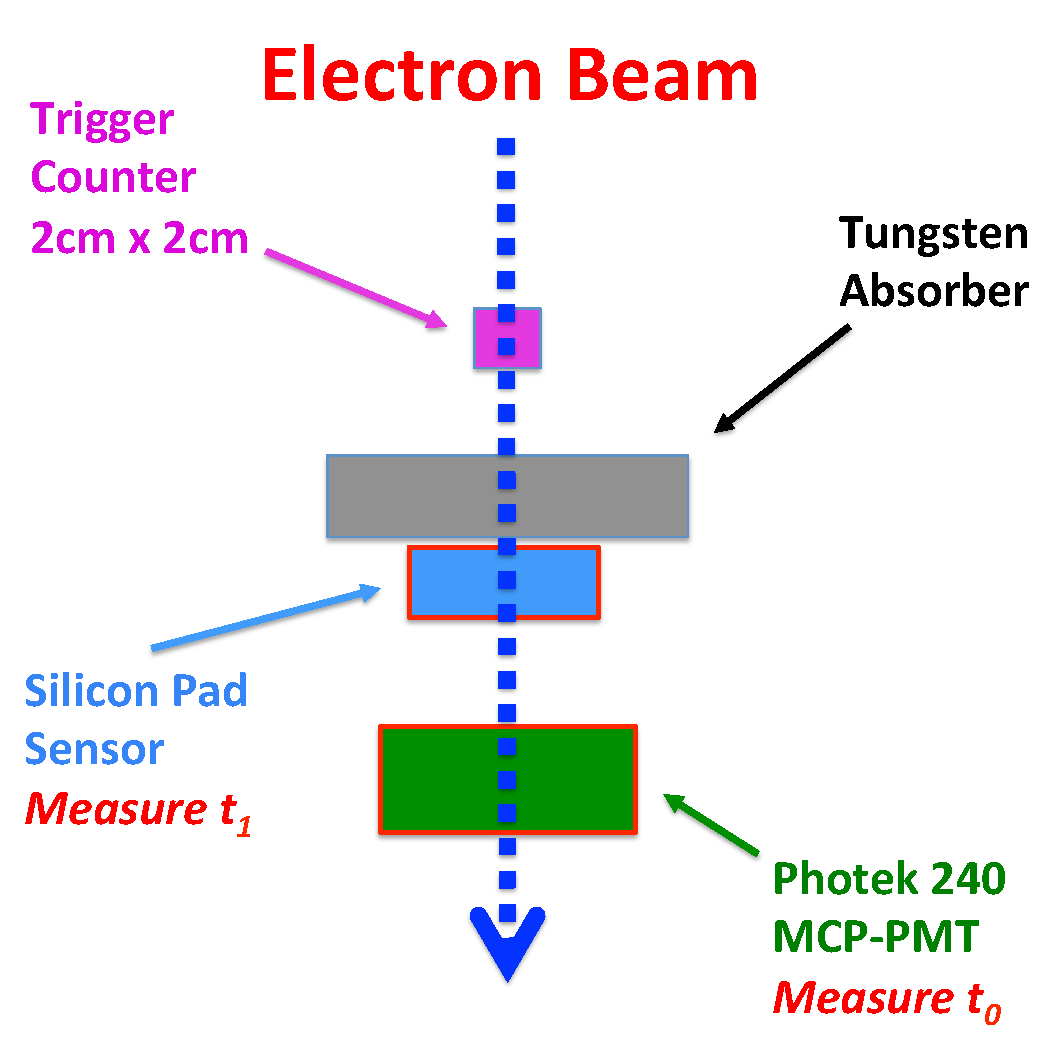
\includegraphics[width=0.65\textwidth]{plots/BeamSchematicDiagram.pdf} 
\caption{A schematic diagram of the test-beam setup is shown. The $t_0$ and $t_1$ are defined in Section~\ref{sec:results}.} 
\label{fig:BeamSchematicDiagram} 
\end{figure} 

\begin{figure}[htbp] 
\centering
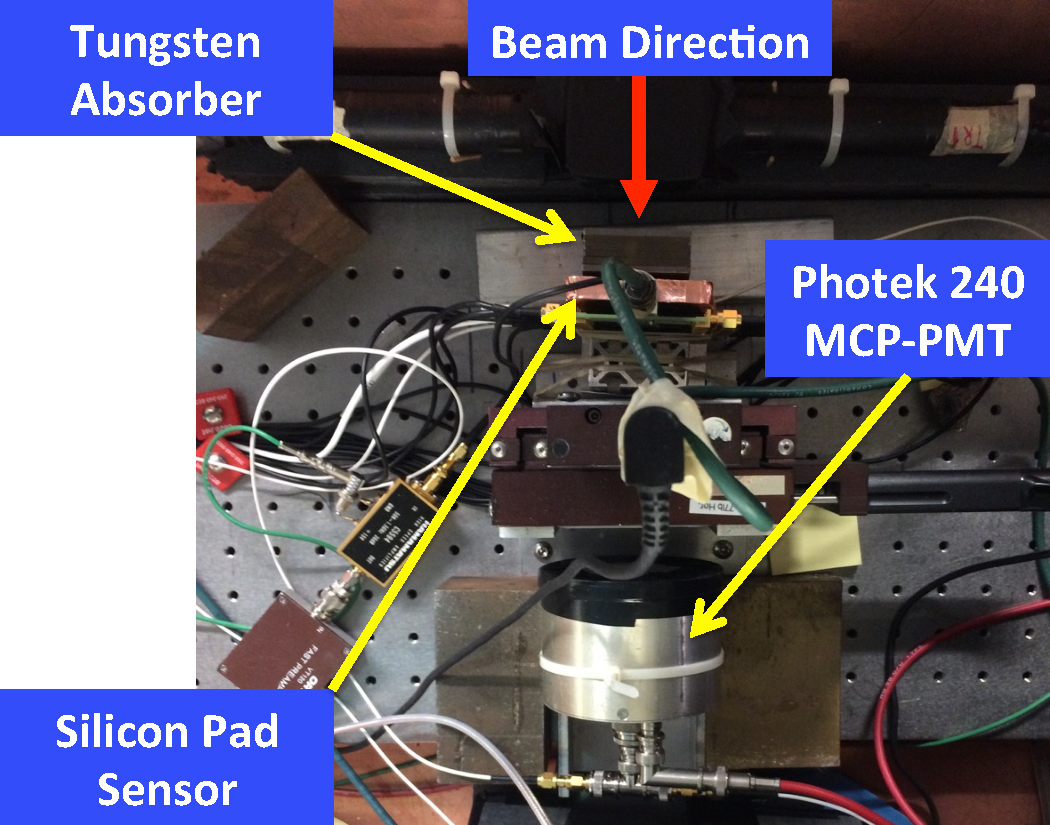
\includegraphics[width=0.65\textwidth]{plots/BeamPhotoDiagram.pdf} 
\caption{Test beam setup.} 
\label{fig:BeamPhotoDiagram} 
\end{figure} 

The DAQ system is based on the CAEN V1742 digitizer board~\cite{CAENDRS}, which
provides digitized waveforms sampled at 5 GS/s. The metal box containing the
silicon sensor was located on a motorized X-Y moving stage allowing us to change
the location of the sensor in the plane transverse to the beam at an accuracy
better than $0.1$~mm. A nominal bias voltage of $500$~V was applied to deplete
the silicon sensor in most of the studies shown below, unless noted otherwise.


\section{Test Beam Measurements and Results} 
\label{sec:results} 

Measurements were performed using the primary 120~GeV proton beam, and secondary
beams provided for the FTBF. Secondary beams with energies ranging from 4
GeV/c$^2$ to 32 GeV/c$^2$ were used. Electron purity for those beams ranges
between $70\%$ at the lowest energy to about $10\%$ at the highest energy.
Stacks of tungsten plates with varying thicknesses were placed immediately
upstream of the silicon device in order to measure the response along the
longitudinal direction of the electromagnetic shower. The radiation length of
tungsten is 3.5~mm, and the Moliere radius is 9.3~mm. The tungsten plate size is
sufficient to fully contain the shower in the transverse dimension. Signals from
the silicon sensor and the Photek MCP-PMT are read out and digitized by the CAEN
V1742 digitizer, and example signal waveforms are shown in
Fig.~\ref{fig:pulses}. The signal pulse in the silicon sensor has a rise time of
about $1.5$~ns, and a full pulse width of around $7$~ns. This rise time is
consistent with a time constant of a silicon sensor coupled to a 50~Ohm amplifier.

\begin{figure}[htbp] 
\centering
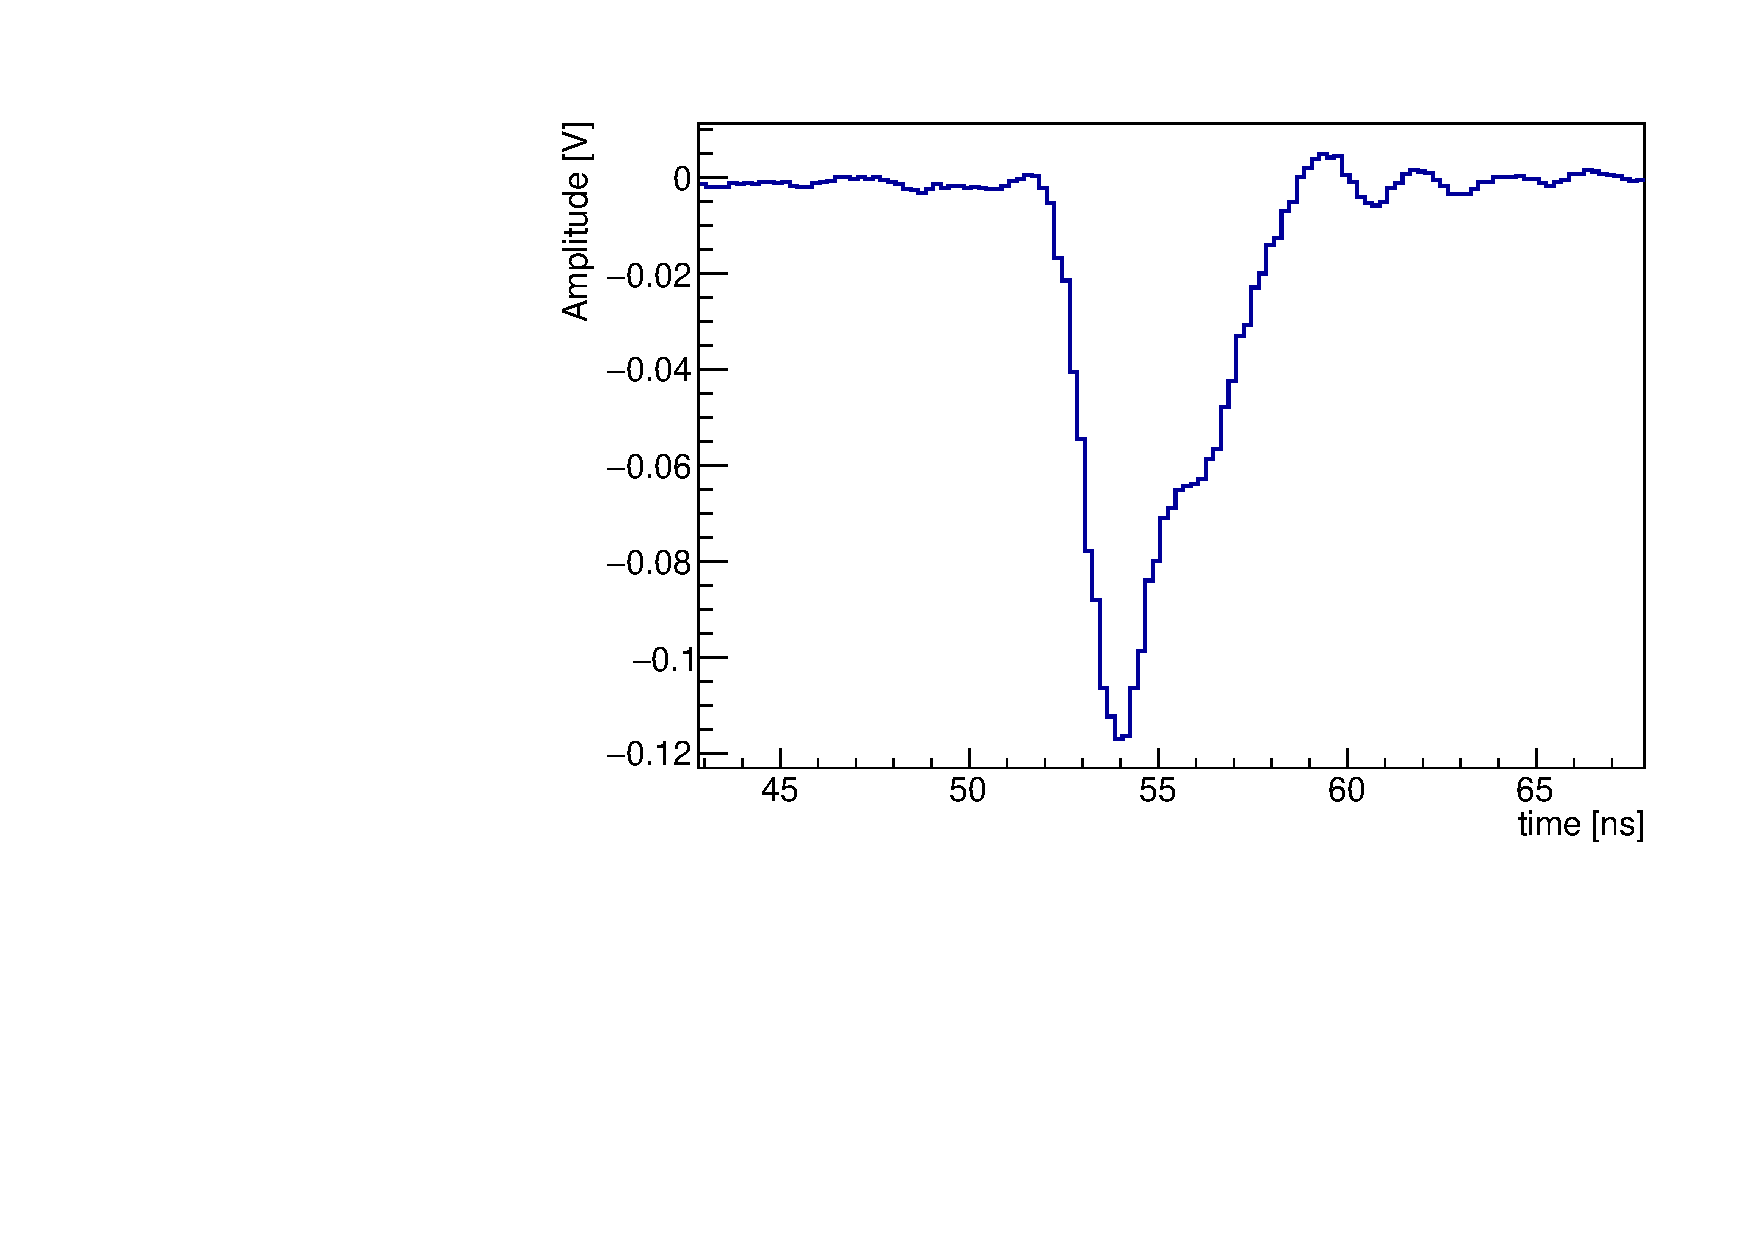
\includegraphics[width=0.45\textwidth]{plots/ExampleSiliconPadPulse_6X0_16GeV.pdf} 
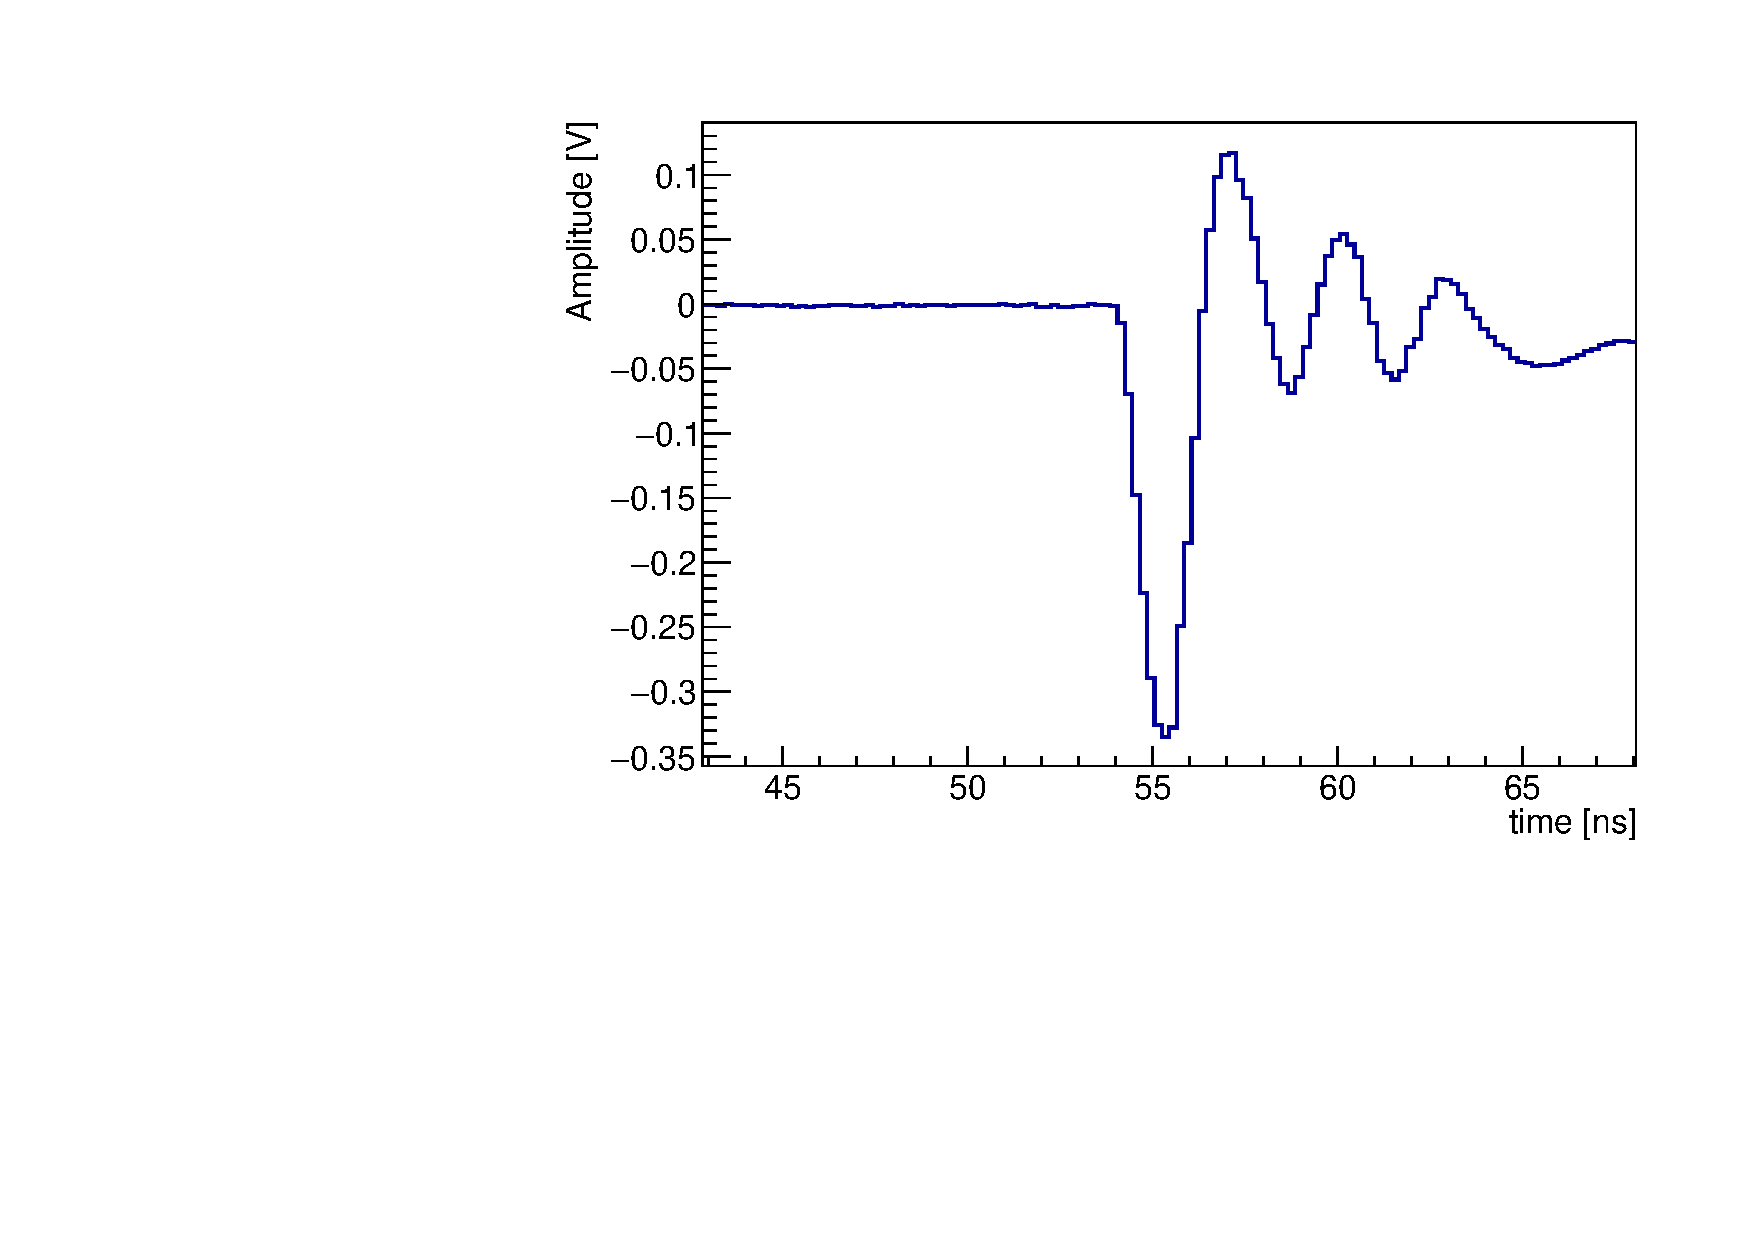
\includegraphics[width=0.45\textwidth]{plots/ExamplePhotekPulse.pdf} 
\caption{Examples of the signal pulse waveform for the silicon sensor (left) and
the Photek MCP-PMT (right) digitized by CAEN V1742 digitizer board. The bias
voltage applied to the silicon pad sensor is~$500$~V.} 
\label{fig:pulses} 
\end{figure} 

The raw waveforms are voltage and time calibrated using the  procedure
described in Ref.~\cite{Kim201467}. The total collected charge for each signal
pulse is computed by integrating a $10$~ns window around the peak of the pulse.
The time for the reference Photek MCP-PMT detector is obtained by fitting the
peak region of the pulse to a Gaussian function and the mean parameter of the
Gaussian is assigned as the timestamp $t_0$. The time for signals from the
silicon sensor is obtained by performing a linear fit to the rising edge of the
pulse and the time at which the pulse reaches 30\% of the maximum amplitude is
assigned as its timestamp $t_1$. We measured the €œelectronic€ time resolution
of the CAEN V1742 digitizer as $\sim$4~ps and neglected its impact on the timing
measurements described below.

Electrons were identified using a combination of the gas Cherenkov counter
provided by the FTBF and the signal amplitude in the Photek detector located further
downstream of the silicon sensor. Electromagnetic showers induced by electrons
produce significantly larger signals in the Photek MCP-PMT, while pions produce
a much smaller signal. After imposing the electron identification 
requirements the electron purity is between $80\%$ and $90\%$ for all beam
conditions. 

We begin by establishing the signal characteristics of a minimum-ionizing
particle (MIP) using beams of 120 GeV protons as well as 8 GeV electrons with no
absorbers upstream of the silicon pad sensor. To separate MIP signals from
noise, we first collect data events with no beam and random trigger. The charge
distribution for these noise runs is presented in Fig.~\ref{fig:noise}. As expected,
the charge distribution is centered at $0$, and the RMS is about
$2$~fC. 

\begin{figure}[htbp] 
\centering
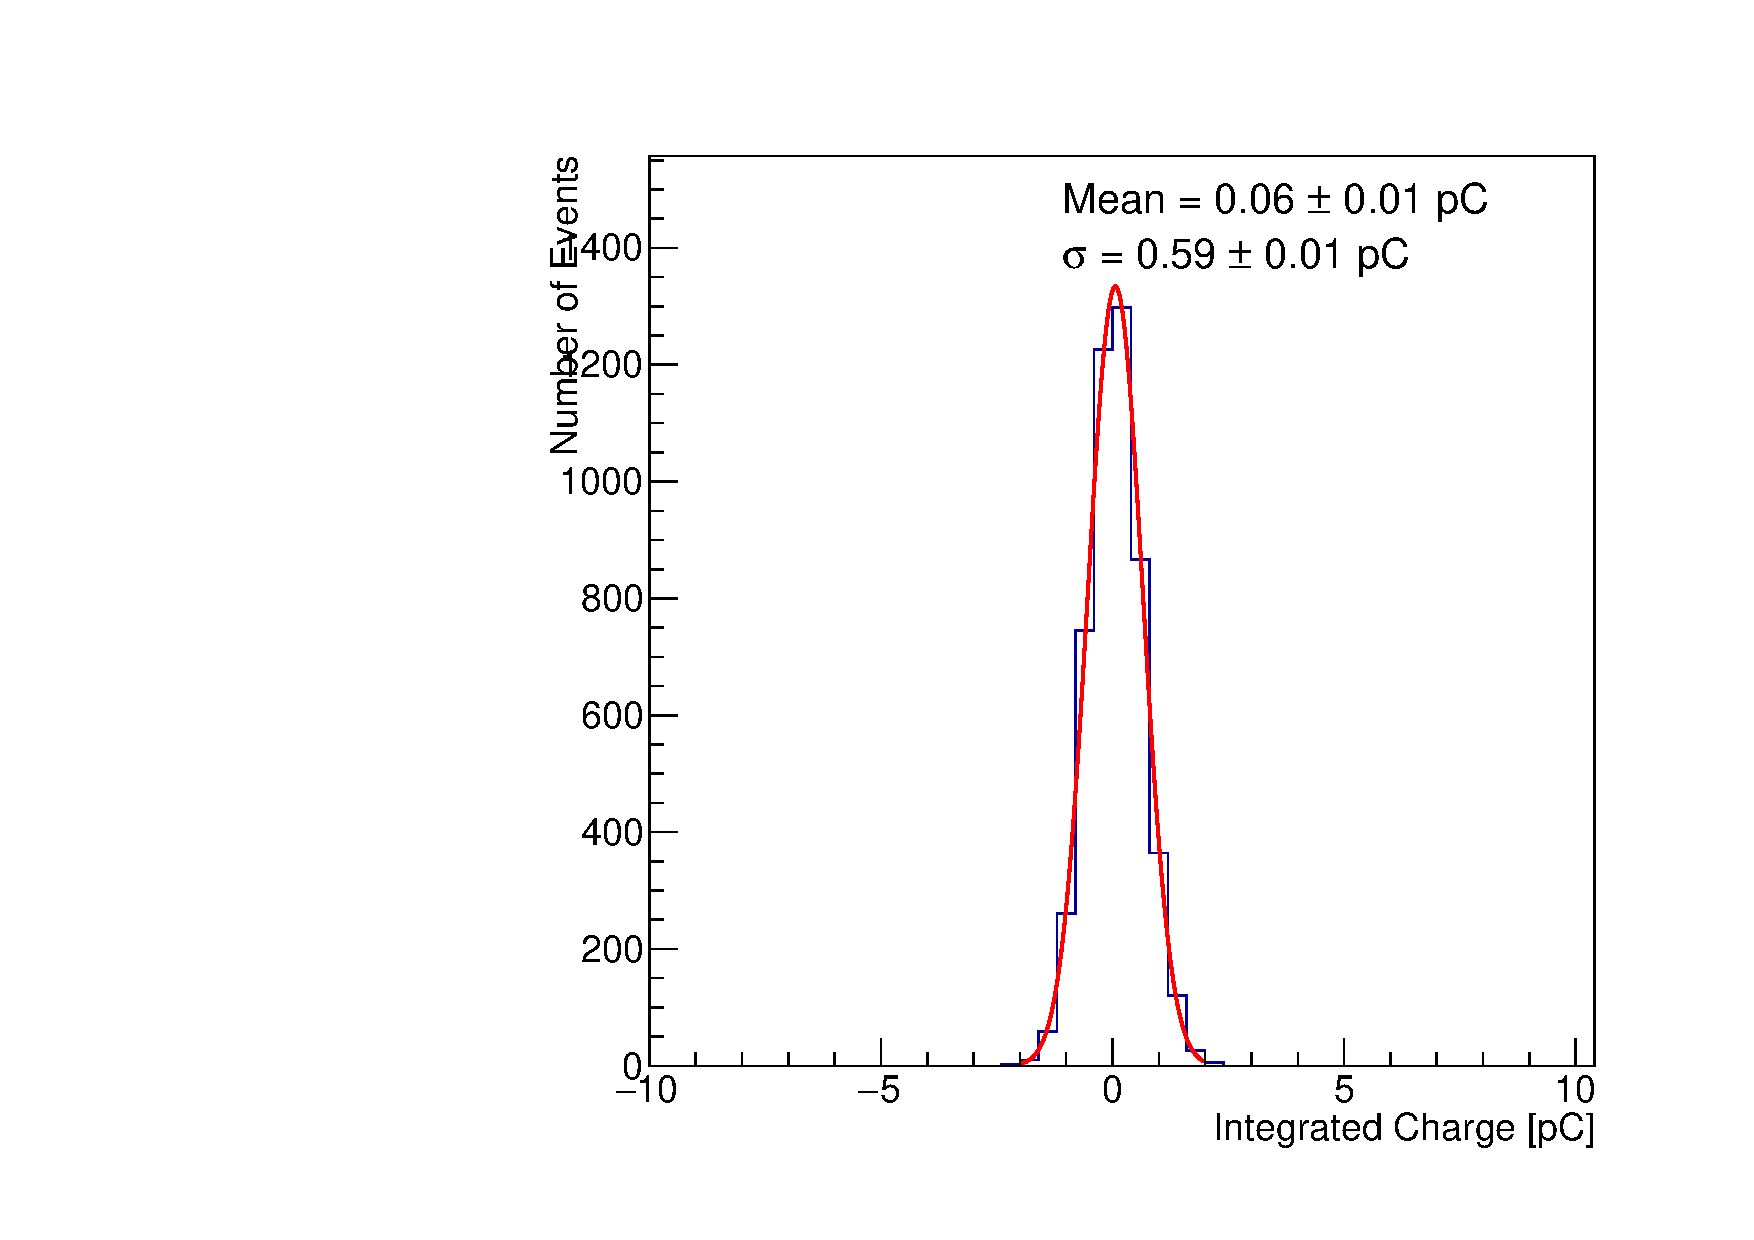
\includegraphics[width=0.45\textwidth]{plots/NoiseNoBeam_charge.pdf} 
\caption{The distribution of charge integrated in the silicon sensor is shown for data events with no beam and random trigger. } 
\label{fig:noise} 
\end{figure} 

In Figure~\ref{fig:MIP}, we show the response of the silicon sensor to the
proton and electron beams without any absorbers upstream. We observe very
similar response for these two cases, and measure an integrated charge of
$4.5$~fC and $5.0$~fC for the proton and electron beams, respectively. The
measured charge is corrected for the gain of the amplifiers and attenuators
used, and hence is the output of the silicon sensor. We expect that a MIP traversing
a silicon sensor of thickness 325~$\mu$m to produce roughly 35,000 electron-hole
pairs, corresponding to a collected charge of about $5$~fC. Thus, our measured value is
in agreement with expectations. Having established the absolute scale of
the  response using MIPs, in our remaining studies we normalize all
charge measurements to the charge integrated in the silicon sensor for one MIP, 
$\mathrm{Q}_{\mathrm{MIP}}$. 

\begin{figure}[htbp] 
\centering
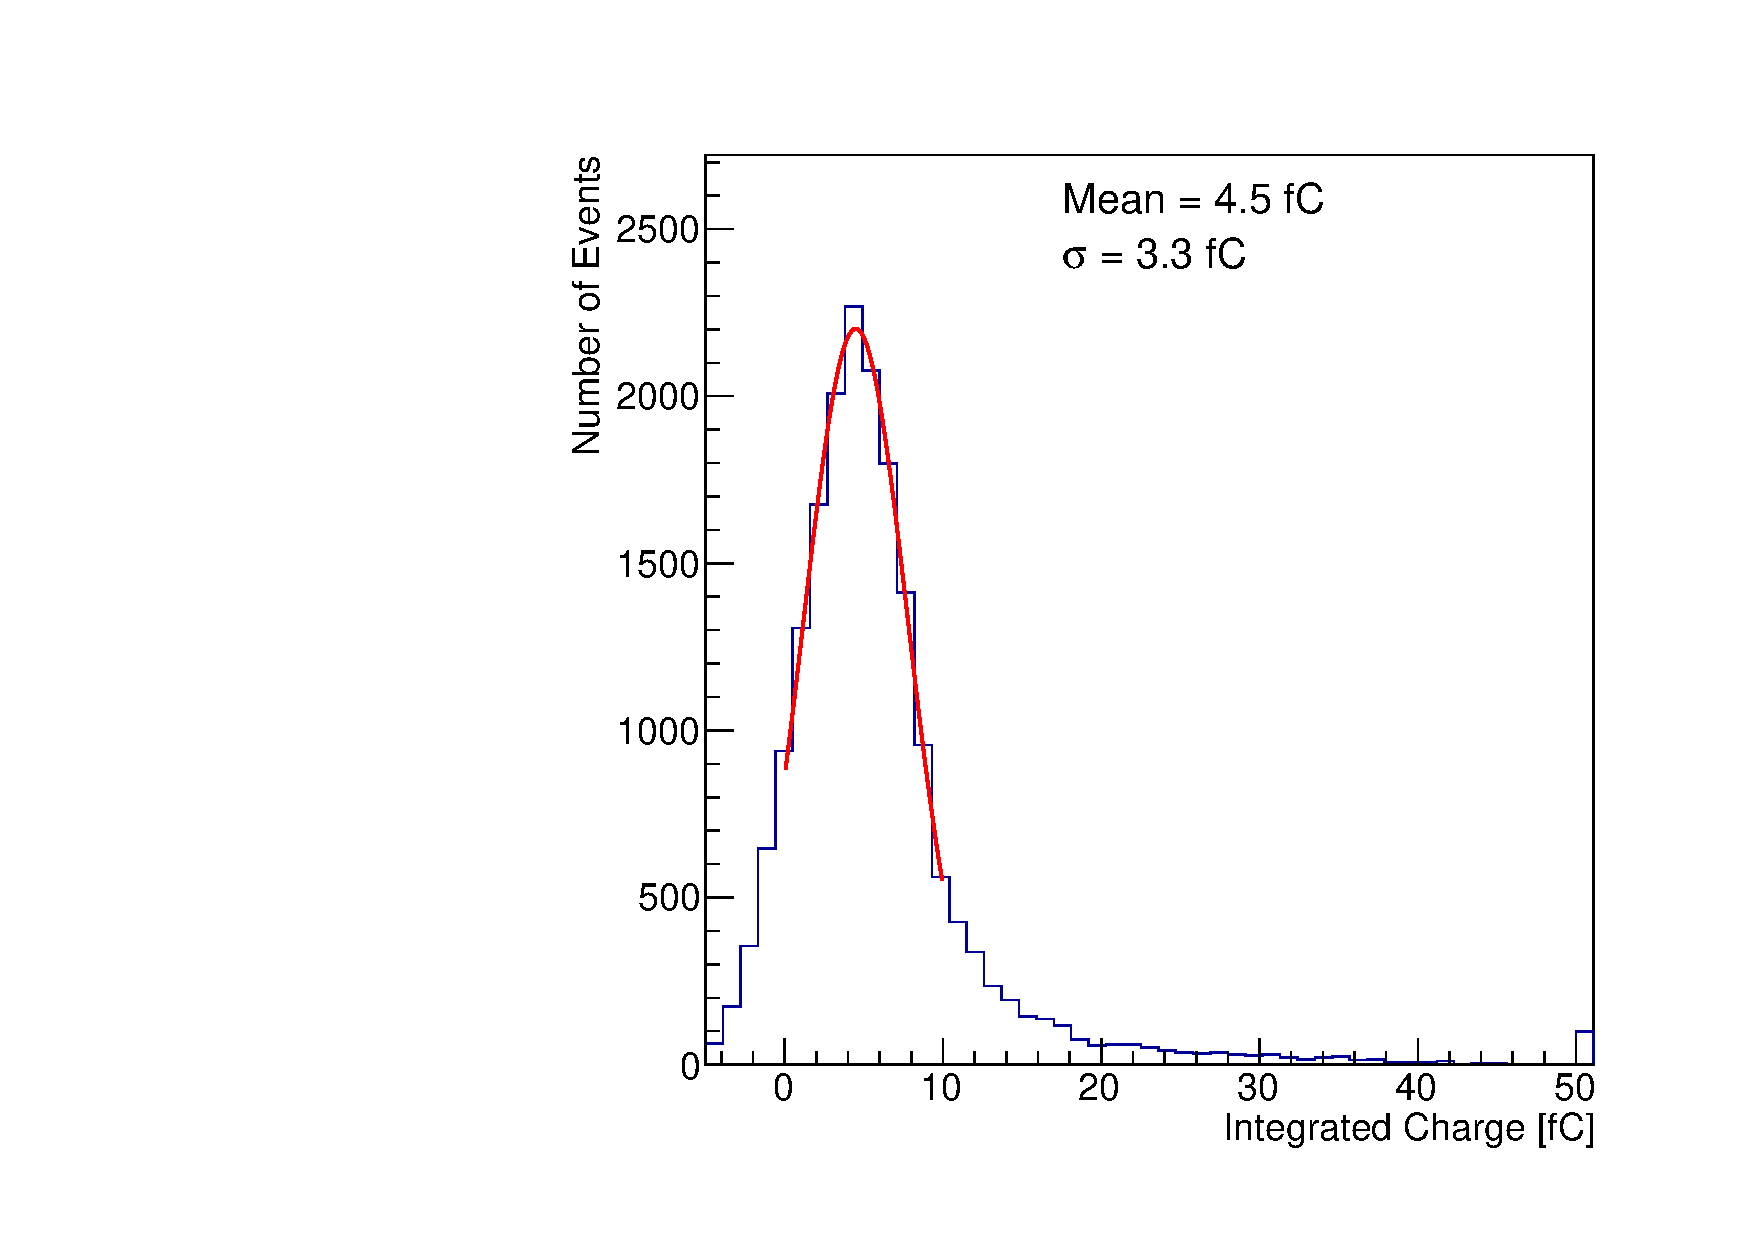
\includegraphics[width=0.45\textwidth]{plots/Proton_charge.pdf} 
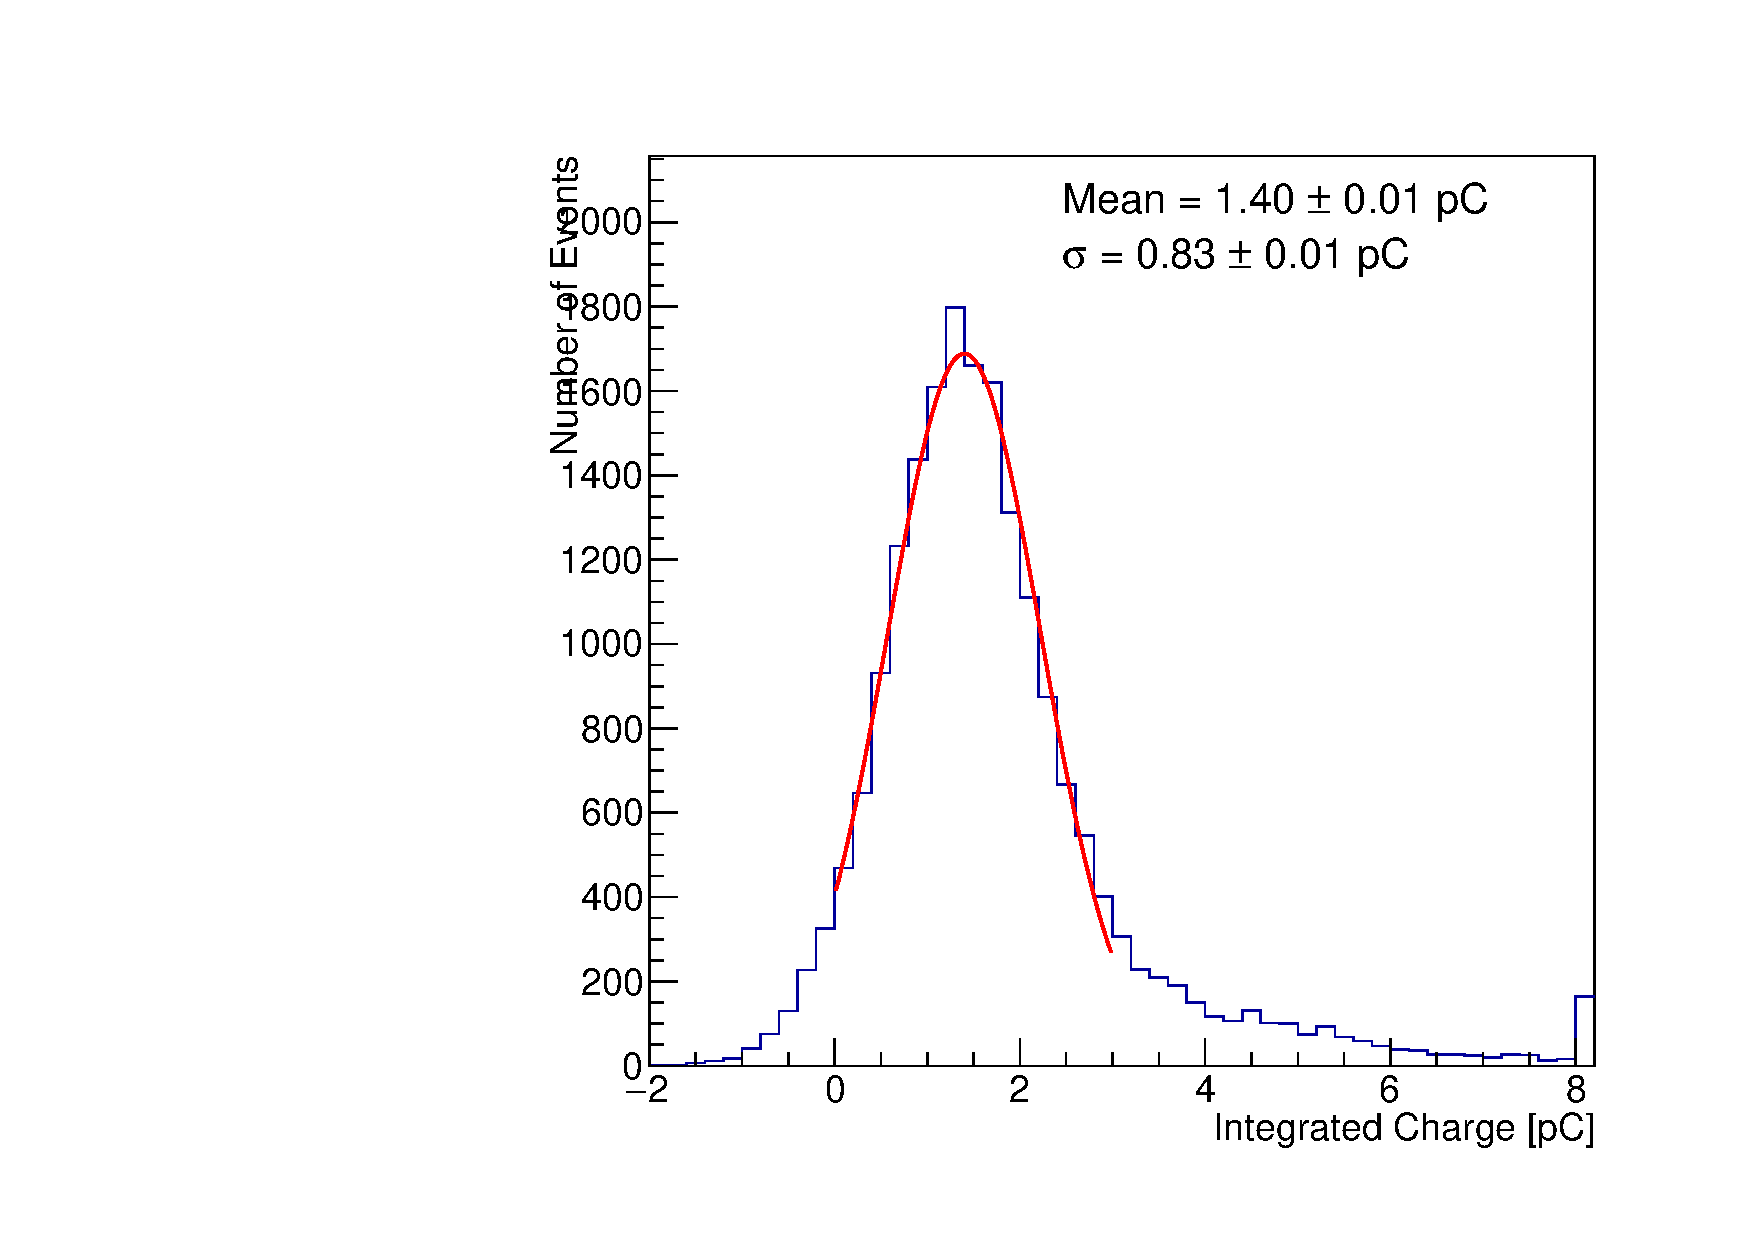
\includegraphics[width=0.45\textwidth]{plots/Electron_0X0_charge.pdf} 
\caption{The distribution of charge integrated in the silicon sensor is shown
for a beam of $120$~GeV protons (left) and $8$~GeV electrons (right) without
any absorber upstream of the silicon sensor. These conditions mimic the response
of the silicon sensor to a minimum-ionizing particle. 
} 
\label{fig:MIP} 
\end{figure} 

We study the response of the silicon sensor to electron beams of various
energies after 6 radiation lengths ($X_0$) of tungsten absorber. The silicon
sensor is expected to be sensitive to the number of secondary electrons produced
within the electromagnetic shower, and therefore its response is expected to
scale up with higher incident electron energy. In
Figure~\ref{fig:ChargeDistributionExample}, we show an example of the integrated
charge distribution measured in the silicon sensor after 6 radiation lengths of
tungsten, for runs with $32$~GeV electrons. We plot the mean and RMS of
these distributions as a function of incident electron beam energy in
Figure~\ref{fig:MIPVsEnergy}. The uncertainties plotted show the RMS of the
charge distribution. We observe a fairly linear depedence between the measured
charge and the incident beam energy, for beam energies between $4$~GeV and
$32$~GeV. 

\begin{figure}[htbp] 
\centering
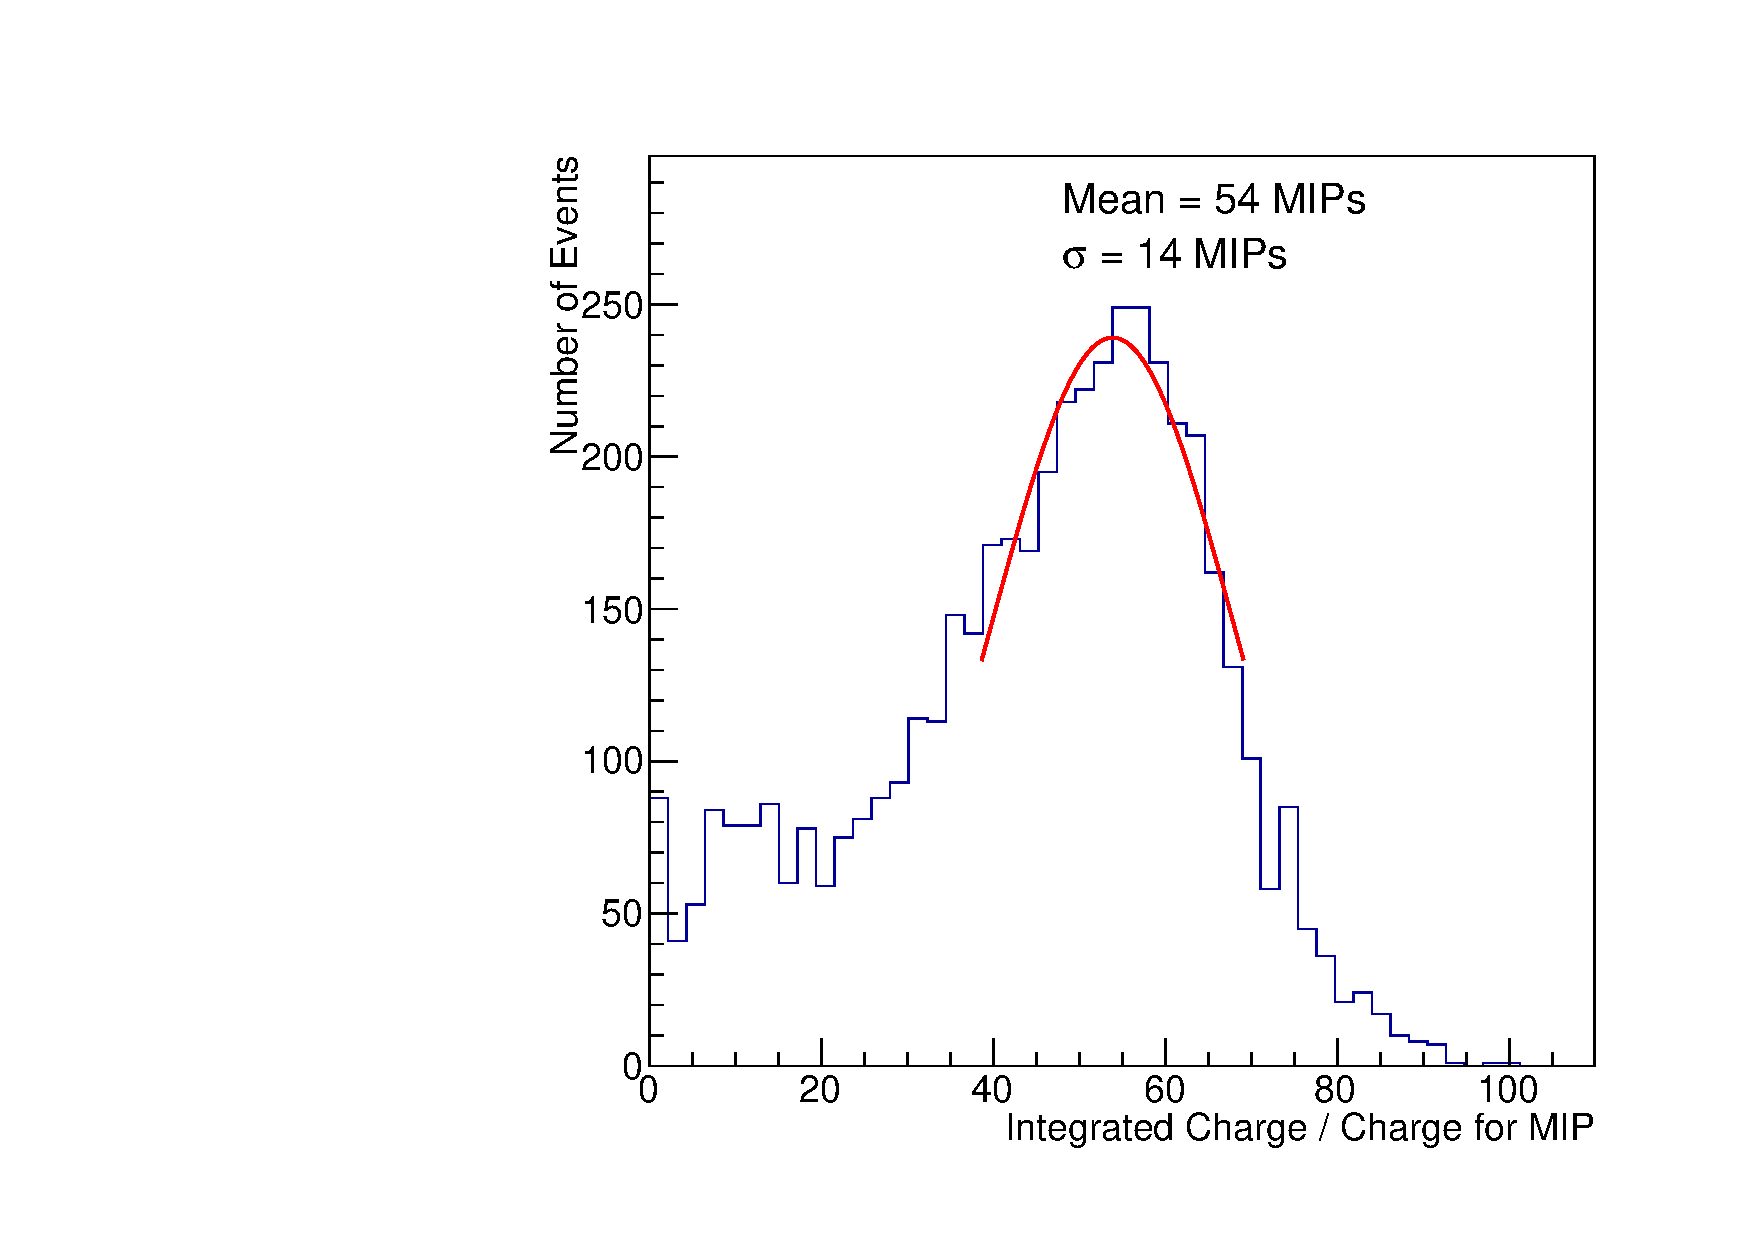
\includegraphics[width=0.49\textwidth]{plots/Electron_6X0_32GeV_chargeMIP.pdf} 
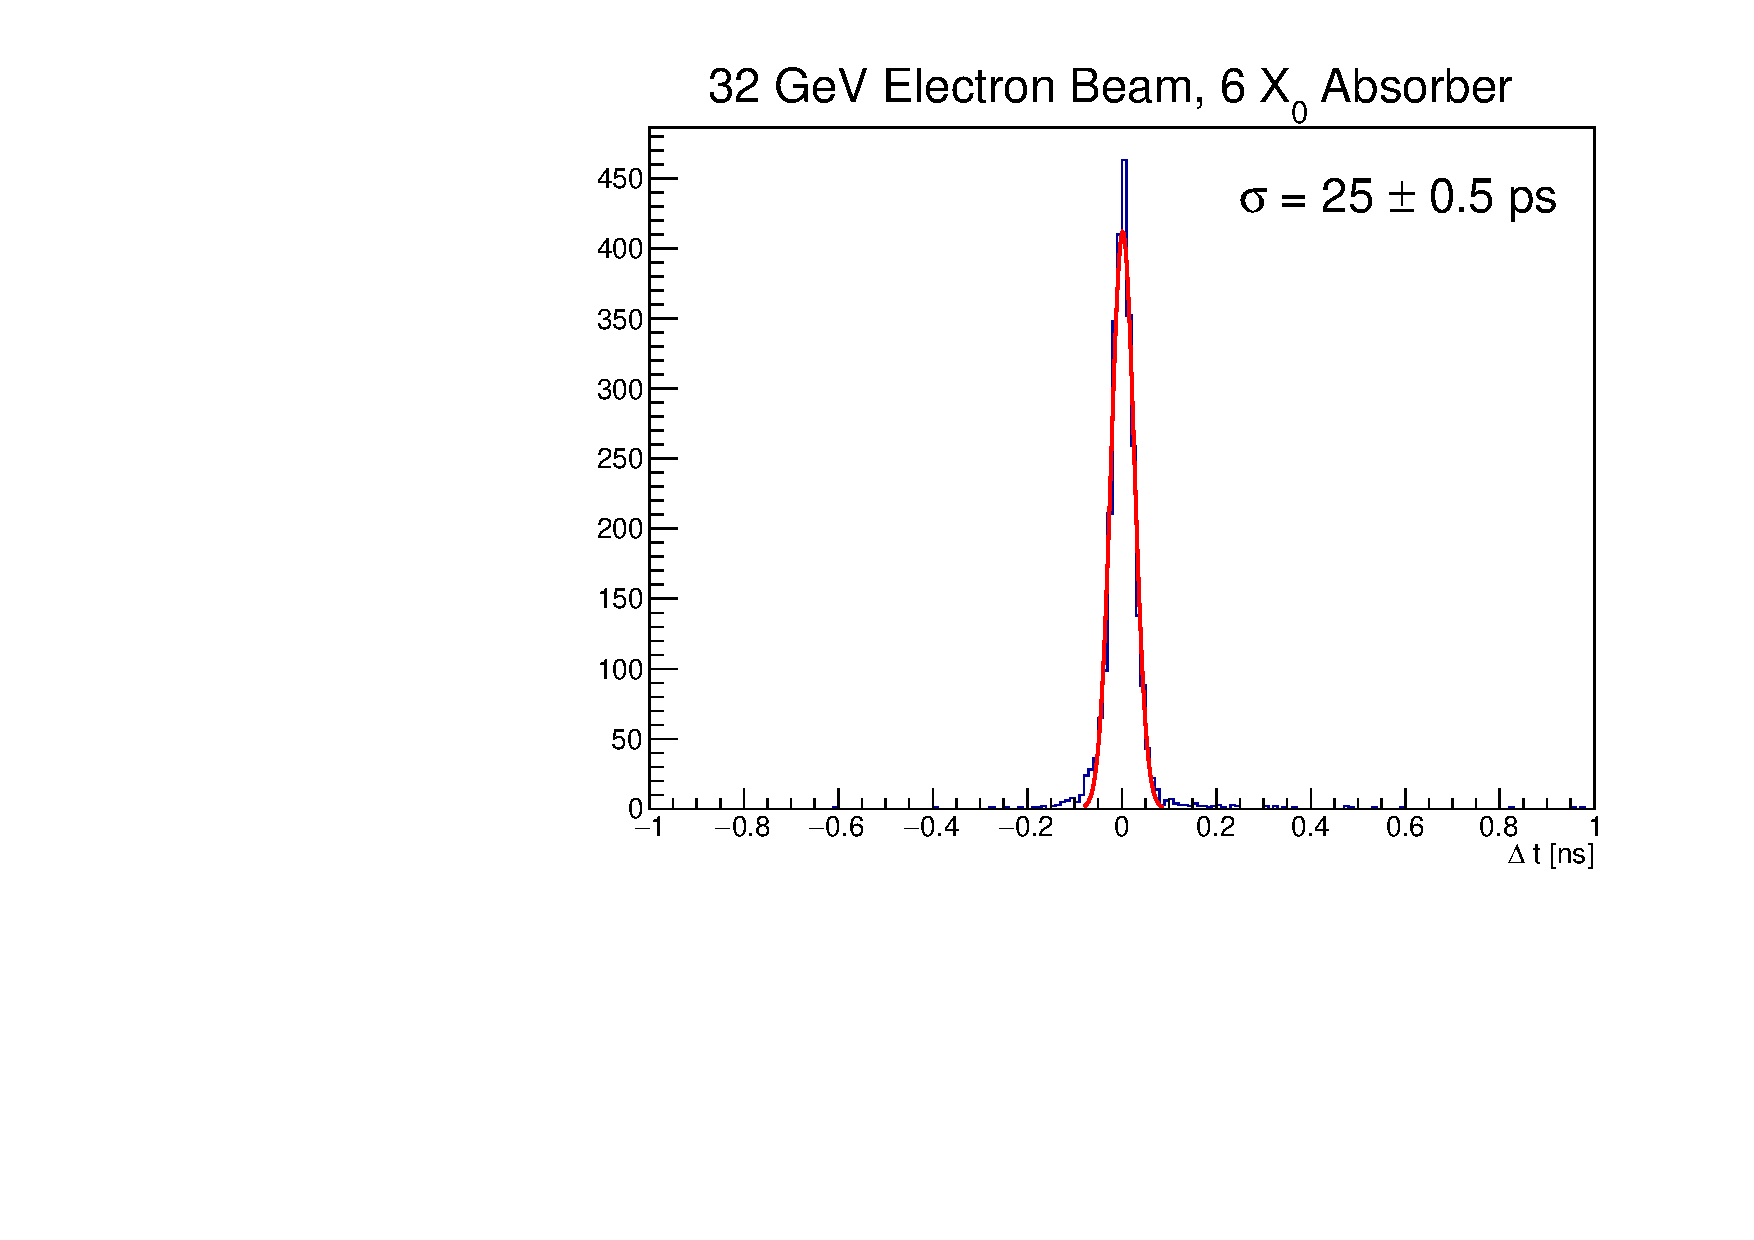
\includegraphics[width=0.50\textwidth]{plots/deltaT_32GeV_6X0.pdf} 
\caption{ Left: An example of the distribution of integrated charge in the silicon
sensor shown in units of charge measured for a MIP. Right: The distribution
of $\Delta$t between the silicon sensor and the Photek MCP-PMT. A 32 GeV
electron beam is used, and the silicon sensor is placed after 6~$X_0$ of tungsten absorber.} 
\label{fig:ChargeDistributionExample}
\end{figure}

\begin{figure}[htbp] 
\centering
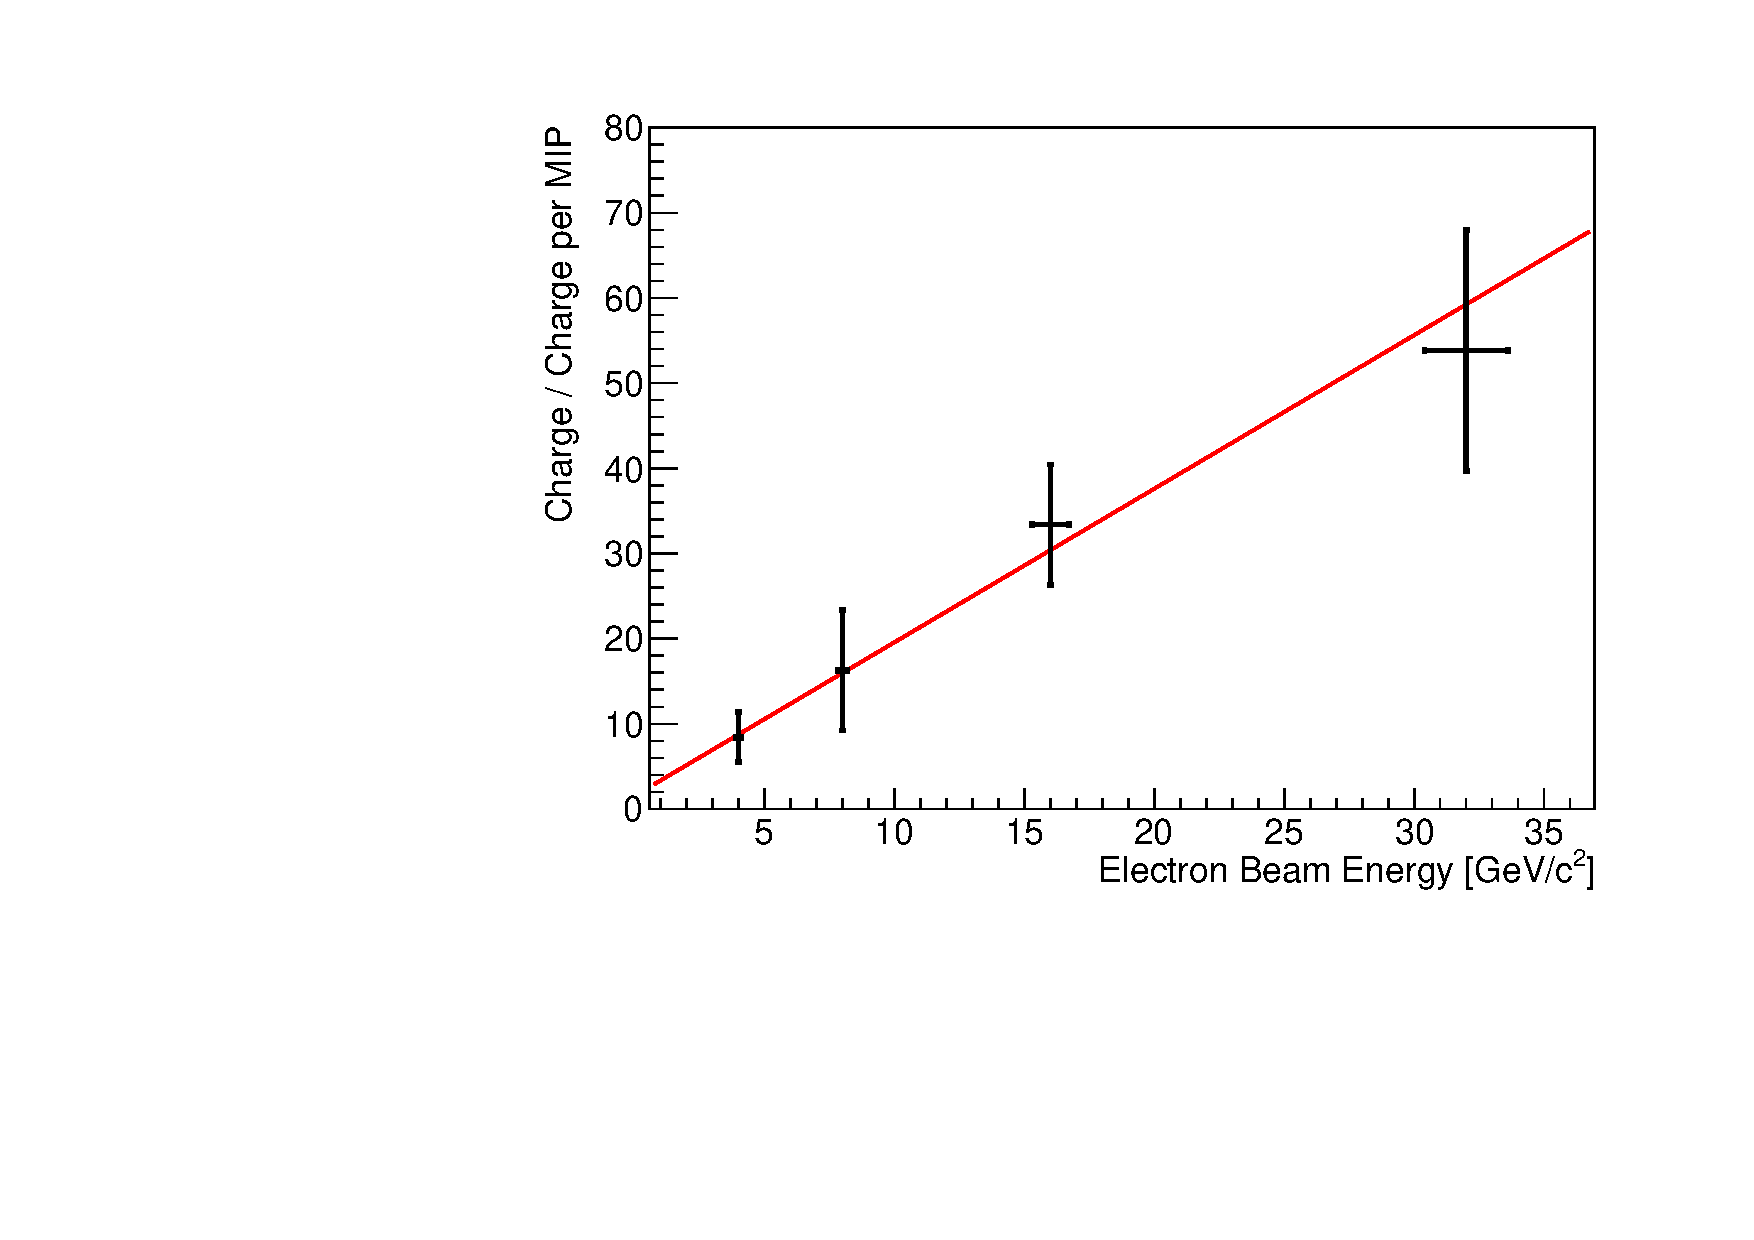
\includegraphics[width=0.49\textwidth]{plots/MIPVsEnergyAt6X0.pdf} 
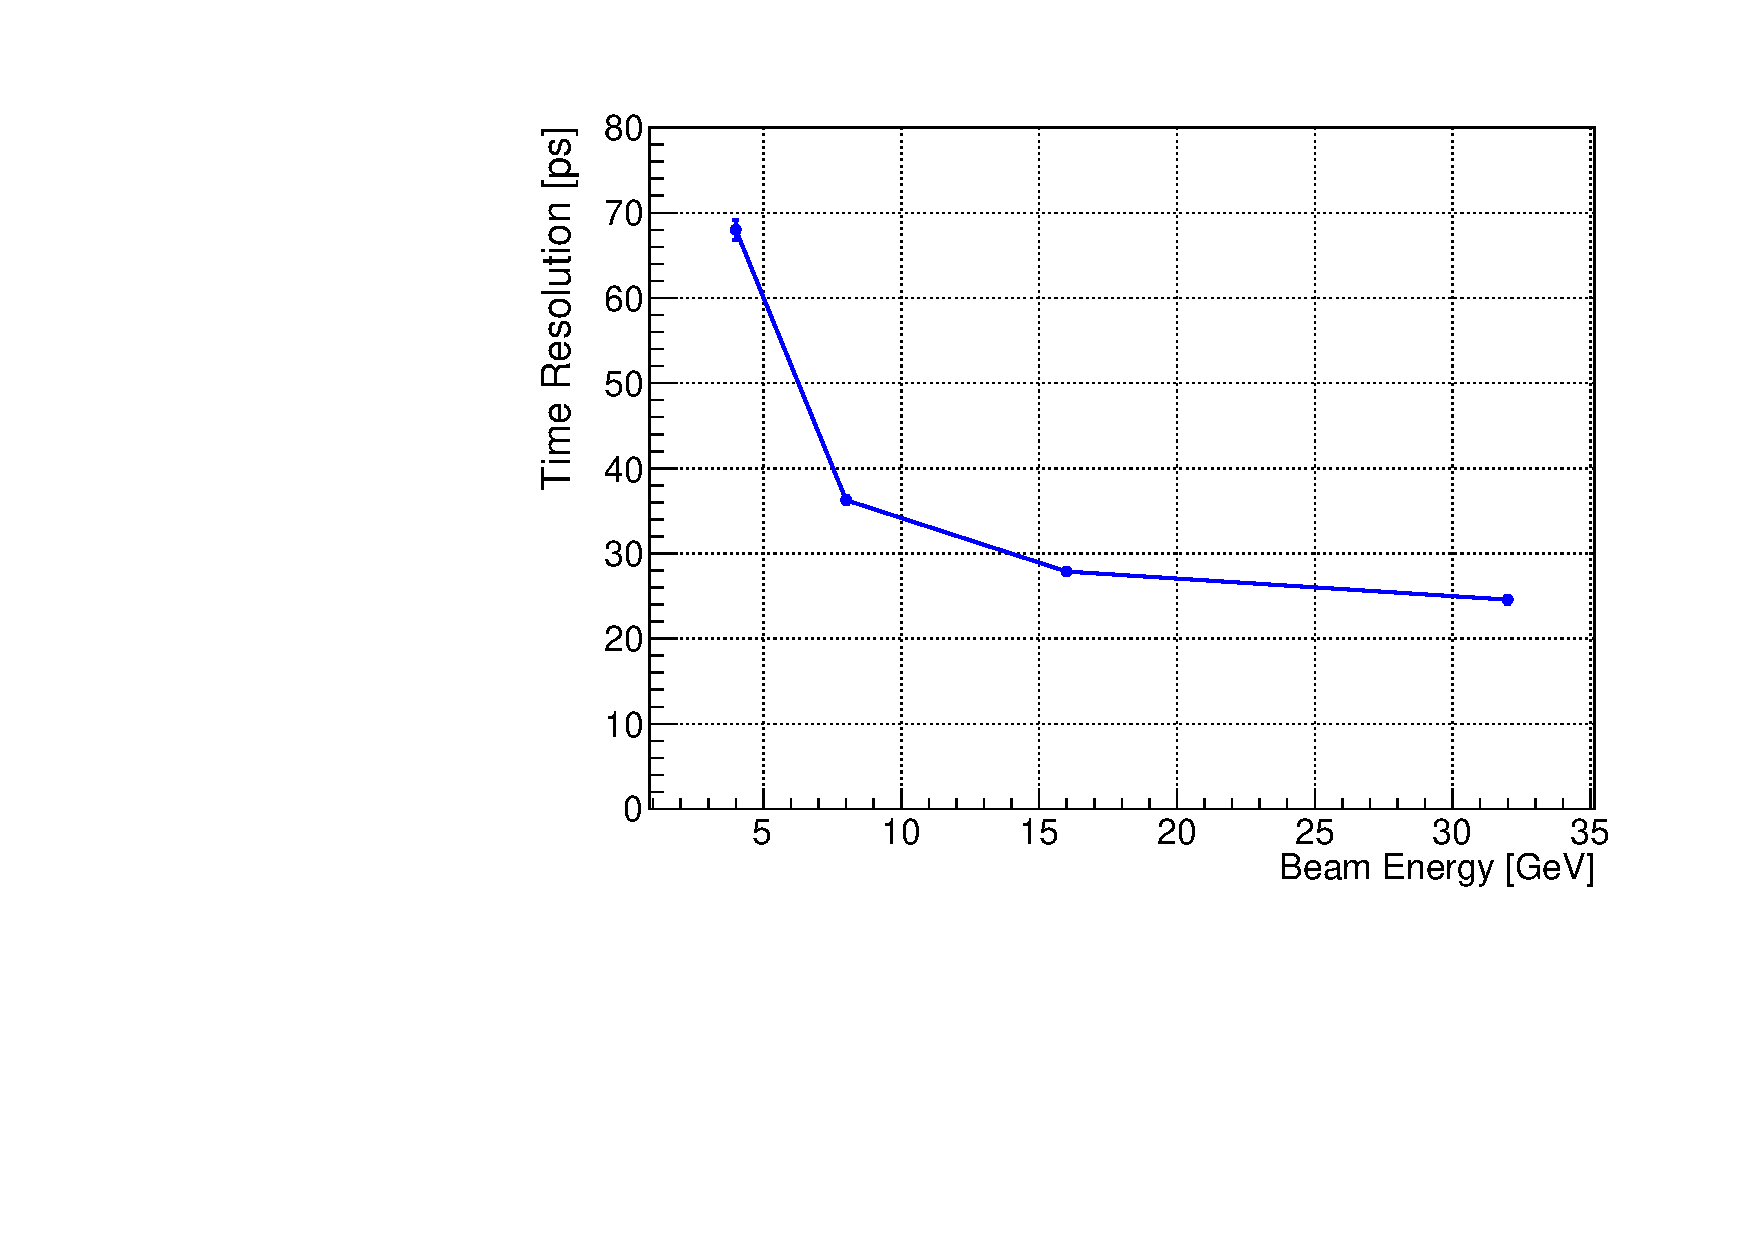
\includegraphics[width=0.50\textwidth]{plots/SigmaT_vs_BeamEnergy_lin30Stamp.pdf} 
\caption{Left: The integrated charge in the silicon sensor expressed in units of the
charge measured for a MIP is shown as a function of the electron beam
energy. The uncertainty bands show the RMS of the measured charge distribution.
The red line is the best fit to a linear function. Right: The measured
time resolution between the silicon sensor and the Photek MCP-PMT reference is
shown as a function of the electron beam energy. } 
\label{fig:MIPVsEnergy} 
\end{figure} 

We also measure the time resolution between the silicon sensor and the Photek
MCP-PMT, by measuring the standard deviation of the gaussian fit to the
distribution of $\Delta t = t_0-t_1$. We observe a systematic dependence of
$\Delta t$ on the total charge measured in the silicon detector, as shown in
Figure~\ref{fig:timewalk}. We perform a correction to $\Delta t$ for each event
using the measured charge in the silicon sensor. The correction is obtained from
a second degree polynomial fit to the distribution of the $\Delta t$ versus
total charge collected in the silicon sensor, as shown in
Figure~\ref{fig:timewalk}. We verify that the correction flattens the dependence
of the time measurement on the integrated charge, as shown on the right panel of
Figure~\ref{fig:timewalk}. An example of a corrected $\Delta t$ distribution for
$32$~GeV electrons after 6 $X_0$ is shown on the right of
Figure~\ref{fig:ChargeDistributionExample}. Other than the electron identification
requirements, no additional selection requirements on the amplitude of the
signal in the silicon sensor were made. The dependence of the measured time
resolution on the beam energy is shown on the right of
Figure~\ref{fig:MIPVsEnergy}. We observe an improvement in the time resolution
as beam energy increases, and achieve a time resolution of $23$~ps for the
$32$~GeV electron beam.

\begin{figure}[htbp] 
\centering
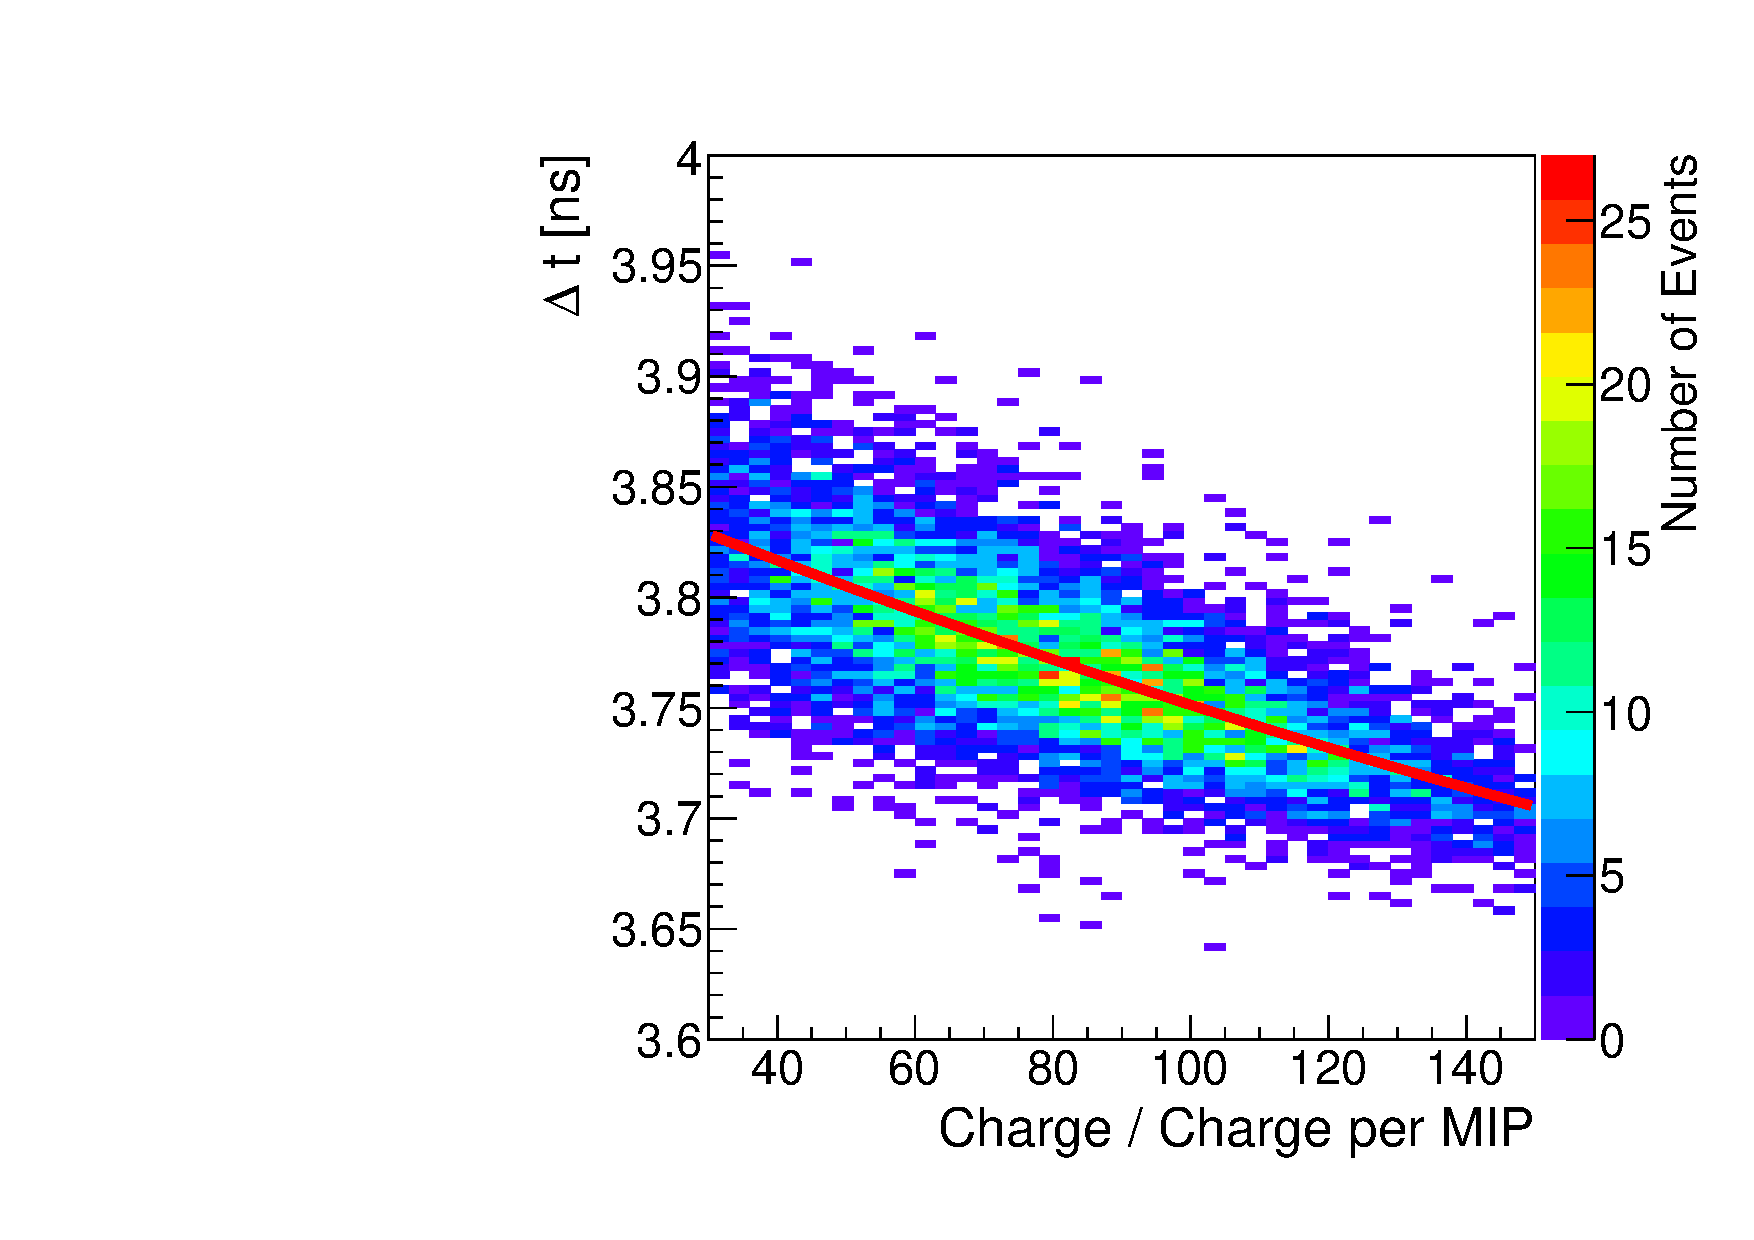
\includegraphics[width=0.49\textwidth]{plots/DeltaT_vs_Charge_Uncorrected.pdf} 
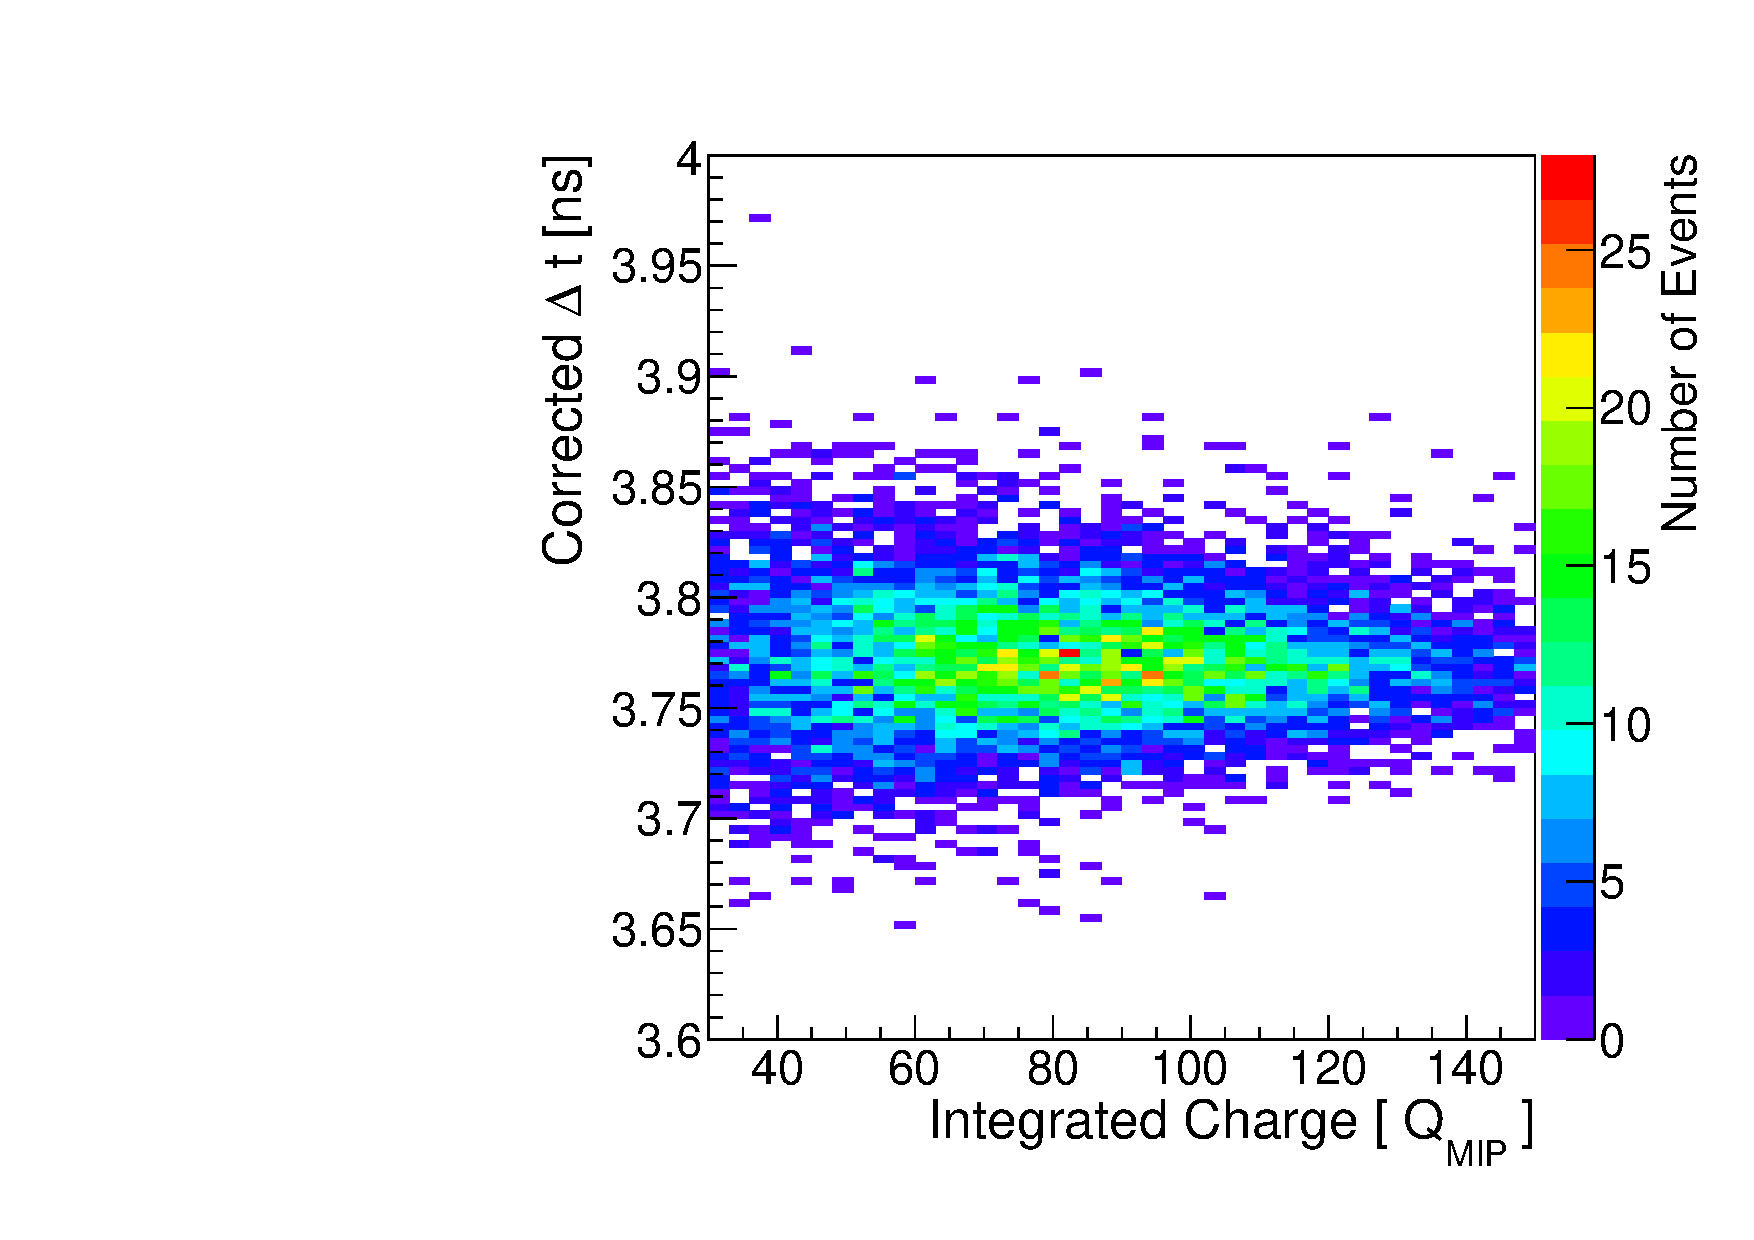
\includegraphics[width=0.5\textwidth]{plots/DeltaT_vs_Charge_Corrected.pdf} 
\caption{ The dependence of $\Delta$t on the integrated charge in the 
silicon sensor is shown on the left. The red curve represents the fit to the
profile plot of the two dimensional distribution, and is used to correct
$\Delta$t for this effect. On the right, we show the corresponding two dimensional
distribution after performing the correction.
} 
\label{fig:timewalk} 
\end{figure} 

Furthermore, we study the response and time resolution of the silicon sensor
along the longitudinal direction of the shower development. We measure the
integrated charge and the time resolution as a function of the absorber
thickness and present the results in Figure~\ref{fig:MIPVsAbsorberAt8GeV}. A
typical longitudinal shower profile is observed, consistent with previous
studies performed using a secondary emission calorimeter prototype based on
MCP's~\cite{MCPShowerMaxPaper}, as well as independent studies of silicon-based
calorimeter prototypes~\cite{Muhuri201424}. We also observe that the time
resolution improves as the shower develops towards its maximum in the
longitudinal direction. 

\begin{figure}[htbp] 
\centering
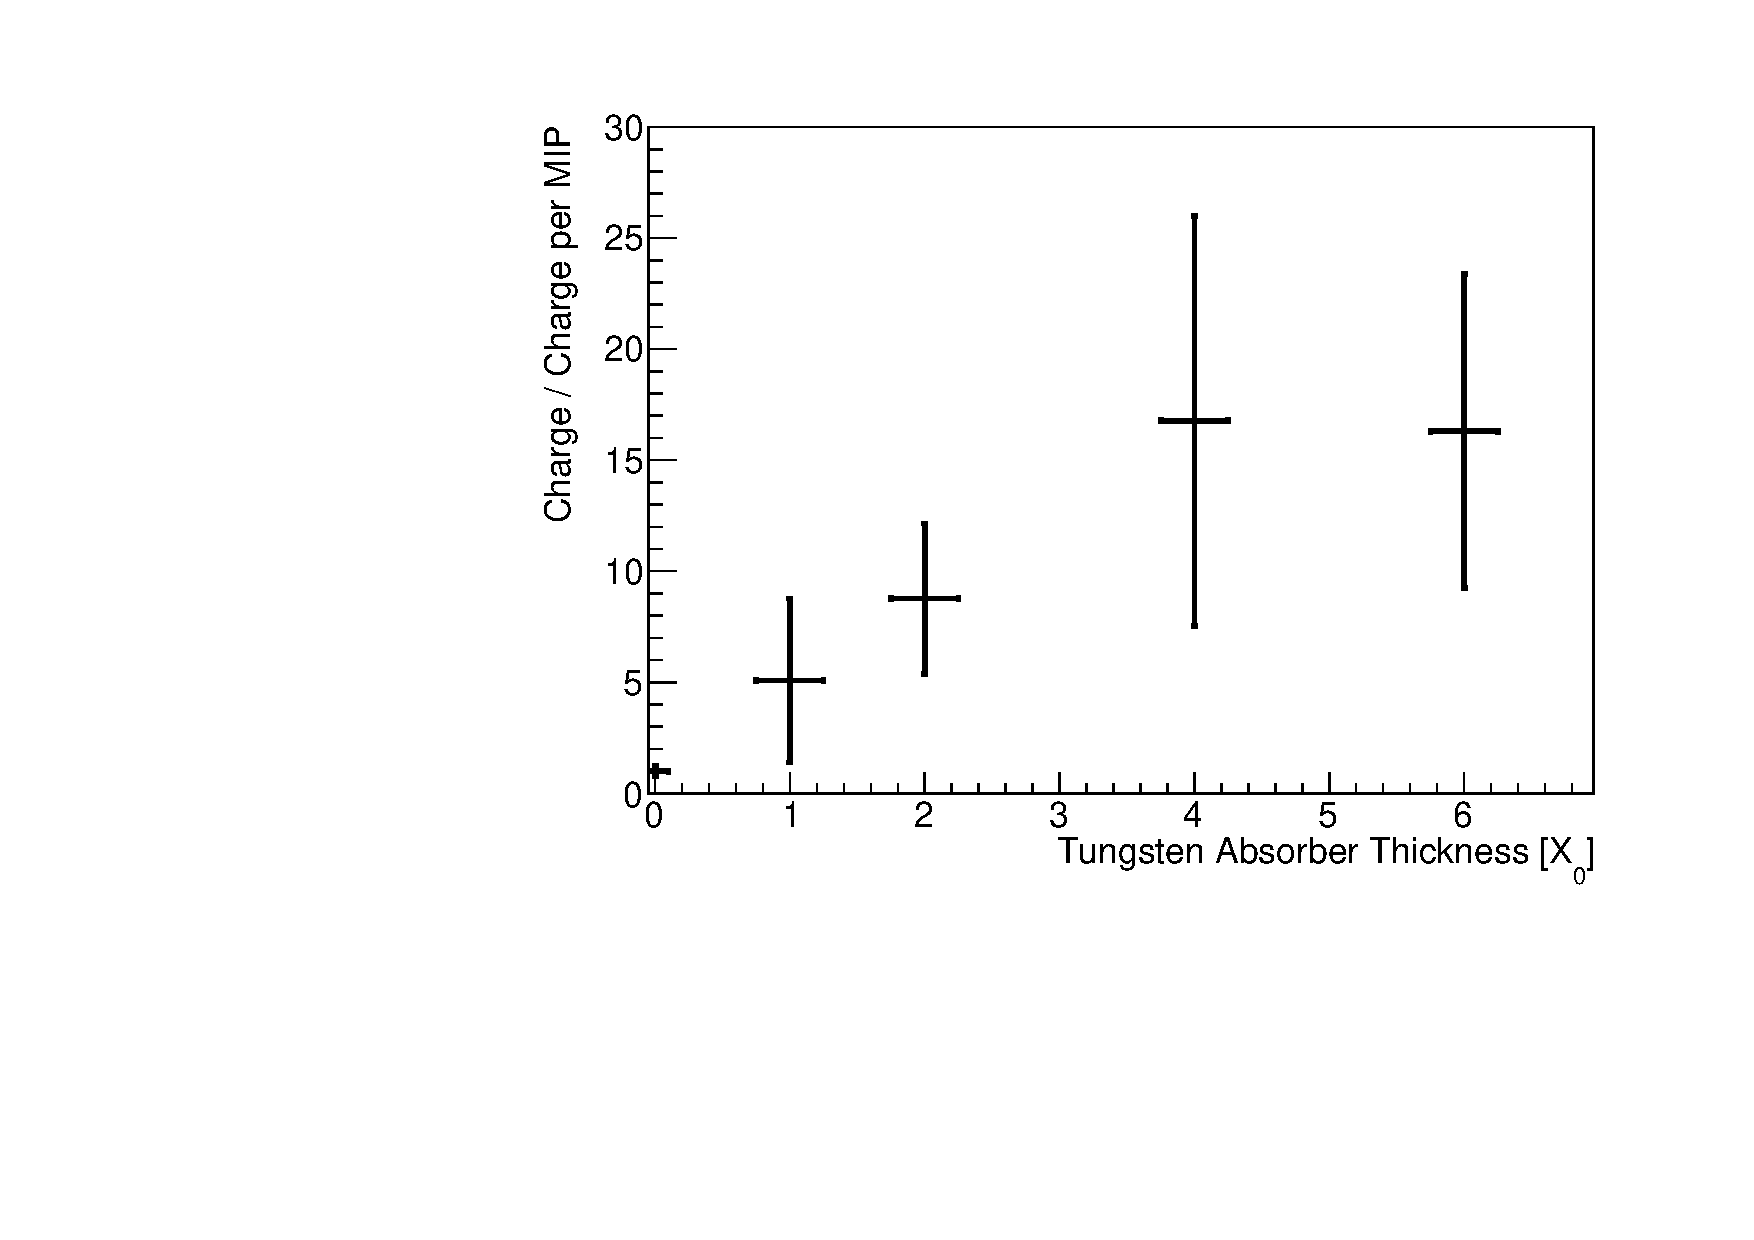
\includegraphics[width=0.49\textwidth]{plots/MIPVsAbsorberAt8GeV.pdf} 
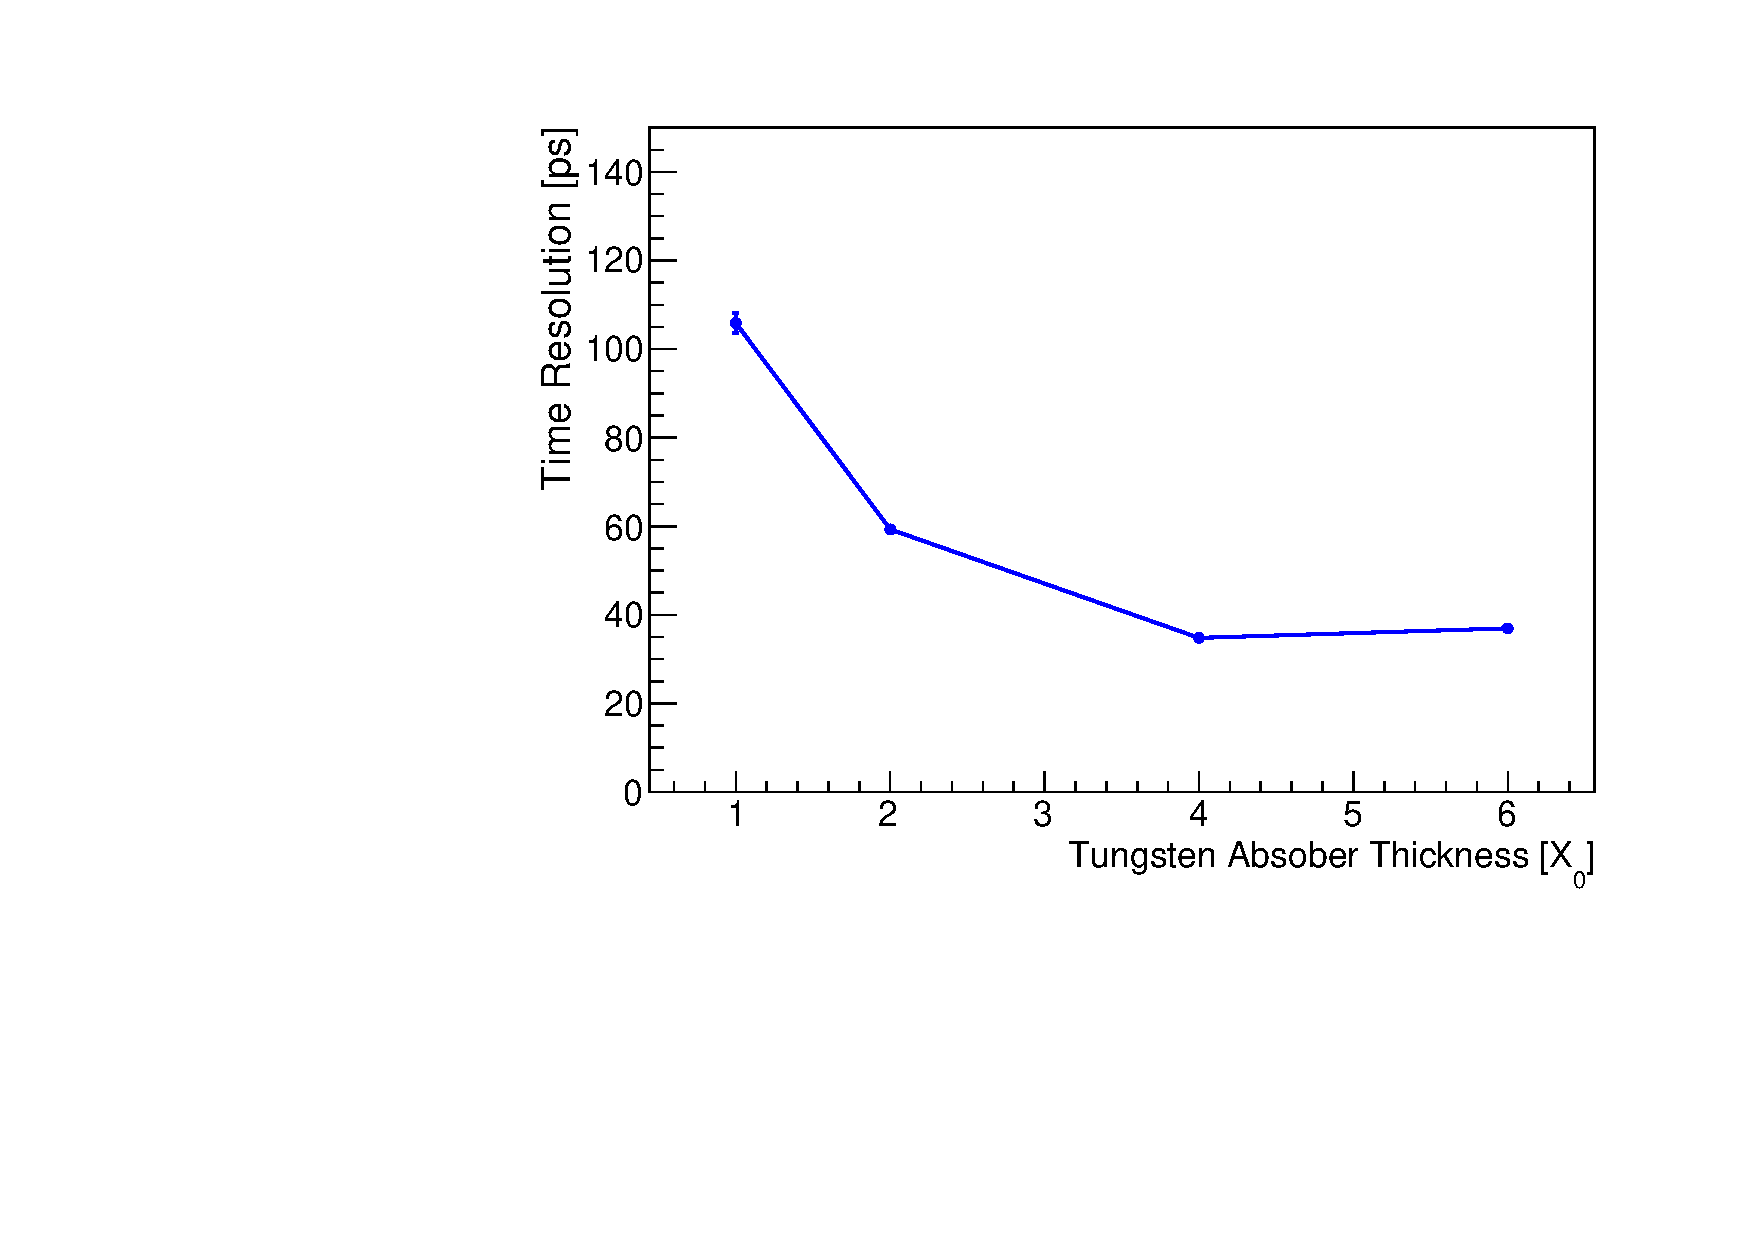
\includegraphics[width=0.5\textwidth]{plots/SigmaT_vs_X0_lin30Stamp.pdf} 
\caption{On the left, the integrated charge in the silicon sensor expressed in units of the 
charge measured for MIPs is shown as a function of the absorber (W) thickness measured in
units of radiation lengths ($X_{0}$). The uncertainty bands show the RMS of the measured charge 
distribution. On the right, the time resolution between the silicon 
sensor and the Photek MCP-PMT reference is shown as a function of the 
absorber thickness.
} 
\label{fig:MIPVsAbsorberAt8GeV} 
\end{figure} 

Finally, we studied the dependence of the time resolution as a function of the
bias voltage applied to deplete the silicon sensor. The measurements are shown
in Figure~\ref{fig:SigmaT_vs_DV_lin30Stamp} for $16$~GeV electrons after
6~$X_0$ of tungsten absorber. We find that the time resolution
improves as the bias voltage is increased, which is expected on the basis of 
increased velocity of electrons and holes in silicon at larger bias voltage. 

\begin{figure}[htbp] 
\centering
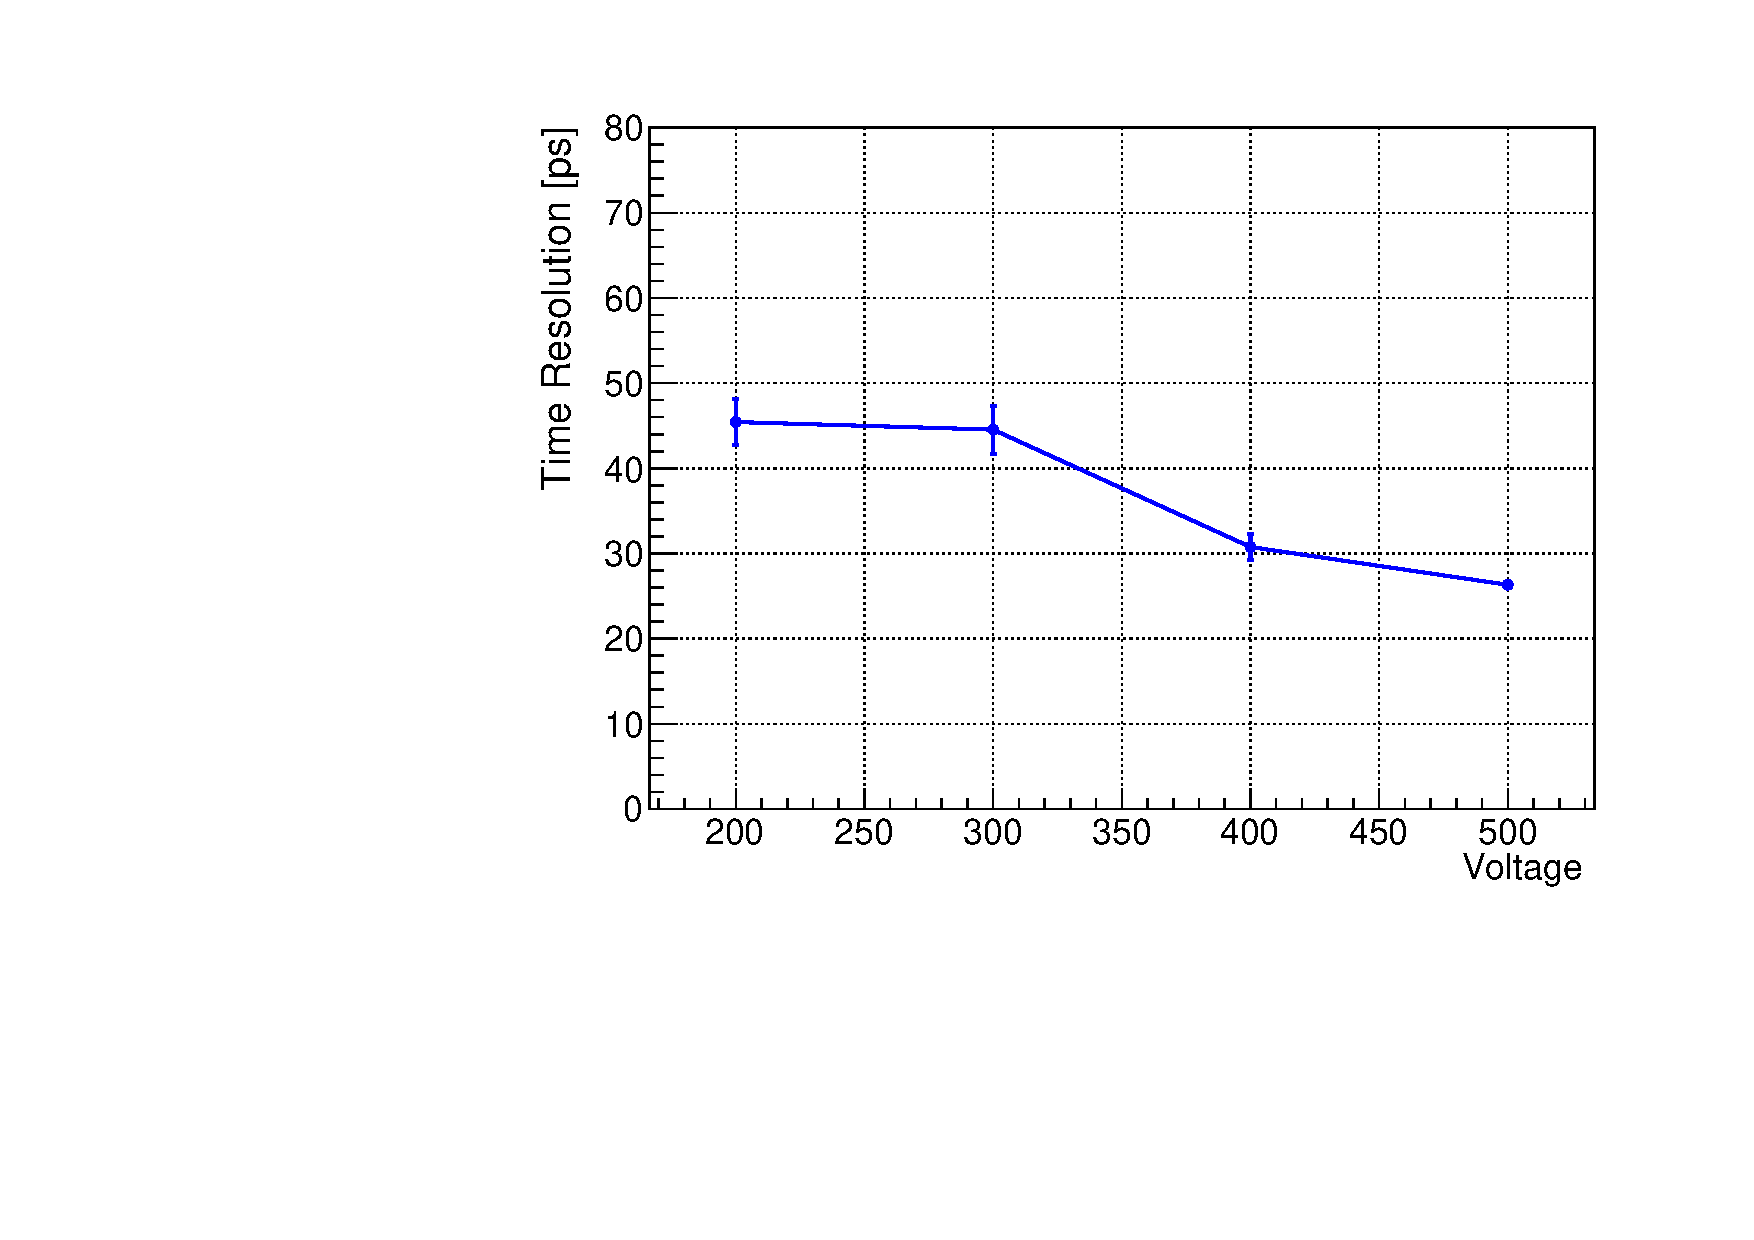
\includegraphics[width=0.8\textwidth]{plots/SigmaT_vs_DV_lin30Stamp.pdf} 
\caption{The time resolution between the silicon sensor and the Photek MCP-PMT 
reference is shown as a function of bias voltage applied on the silicon sensor. } 
\label{fig:SigmaT_vs_DV_lin30Stamp} 
\end{figure} 

\section{Discussion} 
\label{sec:discussion} 

From Figures~\ref{fig:noise}~and~\ref{fig:MIP}, we observe that the noise of the
prototype system is sufficiently low to extract signals from MIPs. Comparing the
RMS of the noise distribution with the mean of the MIP signal, we find a
signal-to-noise ratio around $2$ to $2.5$. A rough estimate from
Figure~\ref{fig:MIP} demonstrates that the efficiency to detect $120$~GeV
protons and $8$~GeV electrons with no absorber present is larger than $80\%$.
Based on the measurements for MIPs, we derive signal distributions for
electromagnetic showers normalized to MIP response, and observe a relatively
linear response to the electron beam energy in the range from 4~GeV to 32~GeV
after 6 $X_0$ of tungsten absorber, as shown in Figure~\ref{fig:MIPVsEnergy}. We also
measure a longitudinal shower profile in Figure~\ref{fig:MIPVsAbsorberAt8GeV}
that is consistent with similar past measurements.

With regards to the timing measurements, we begin with some general considerations.
An electric field applied to silicon results in a built-in junction voltage
($\sim 0.6$~V) which is typical of silicon diodes. The high electric field in silicon
leads to total depletion as all free charge carriers are removed. 
When charged particles pass through the totally depleted region in silicon, 
it ionizes atoms and produces electron-hole pairs which serve as charge carriers.
The electrons are collected on positive electrode and the holes are collected
on the negative electrode. The time and jitter associated with relativistic particles 
traversing through the silicon material can be neglected as it takes 
less than $1$~ps for relativistic particles to pass through the full $300$~$\mu$m
of silicon material. At high electric field (more than $10^{5}$~V/cm), the mobility 
of carriers attain a constant drift velocity of $1\mu$m$/10$~ps in the silicon 
material~\cite{Ronzhin2015,spieler2005semiconductor}. The time required to collect all ionization electrons
produced by a charged particle traversing the $300\mu$m is about $3$~ns.
The electrons produced closer to the positive electron are collected first and are
most relevant for the time stamp assignment. The time needed to collect the electrons
produced in the last $3\mu$m of silicon is about $30$~ps, and roughly sets the scale
of the time measurement.

Our results show that the time stamp associated with electromagnetic 
showers induced by electrons with energy between $20$~GeV and $30$~GeV 
can be measured with a precision better than $25$~ps. Subtracting for the resolution
of the reference Photek MCP-PMT detector yields a precision better than $20$~ps. 
Moreover, we observe an improvement of the time resolution with the energy of 
the electron, and more generally with an increase in the signal amplitude. 
These measurements demonstrate that a calorimeter based on silicon sensors as
the active medium can achieve intrinsic time resolution at the $20$~ps level, as long
as noise is kept under control. Time jitter arising from intrinsic properties of the
silicon sensor is demonstrated to be well below the $20$~ps level.

\section{Conclusion}
\label{sec:conclusion} 

We obtained a best time resolution measurement for silicon sensors of $23$~ps,
using a beam of $32$~GeV electrons and with the silicon sensor placed after 6 radiation
lengths of tungsten absorber. Based on our calibration data for the response of the
silicon sensor to MIPs, this measurement corresponds roughly to 
$54$ secondary particles registered from the electromagnetic shower. 
We observe a roughly linearly increasing response as the energy of the electron beam
is increased, and we observe a longitudinal shower profile consistent with similar 
past measurements. This result yields further encouragement to use silicon as
active layers in calorimeters, as is planned for example for the CMS Phase 2 
upgrade~\cite{Butler:2020886}, and explicitly demonstrates the opportunity 
to use silicon for timing measurements in future calorimeters. In the future, we plan to 
extend our studies to more realistic prototypes covering larger transverse and longitudinal 
regions of the electromagnetic shower and using multiple channels. 


\section{Acknowledgements} We thank the FTBF personnel for very good beam 
condition during our test beam run. We also appreciate the technical support of 
the Fermilab SiDet department for the production of high quality silicon samples. 

\bibliography{SiliconCalorimeter}{}
\bibliographystyle{ieeetr} 

\end{document}





















